\documentclass[12pt]{book}
\usepackage{mathptm,times,color}
\usepackage[pdftex]{graphicx}
\usepackage{hyperref}
\usepackage{multirow}

\renewcommand{\bibname}{References}

%\usepackage{eso-pic}
%\usepackage{graphicx}
%\usepackage{color}
%\usepackage{type1cm}


%\makeatletter
%   \AddToShipoutPicture{%
%     \setlength{\@tempdimb}{.5\paperwidth}%
%    \setlength{\@tempdimc}{.5\paperheight}%
%   \setlength{\unitlength}{1pt}%
%  \put(\strip@pt\@tempdimb,\strip@pt\@tempdimc){%
%     \makebox(0,0){\rotatebox{45}{\textcolor[gray]{0.75}{\fontsize{8cm}{8cm}\selectfont{DRAFT}}}}}}
%\makeatother

\setlength{\textwidth}{6.5in}
\setlength{\textheight}{9.0in}
\setlength{\topmargin}{0.in}
\setlength{\headheight}{0.in}
\setlength{\headsep}{0.in}
\setlength{\parindent}{0.25in}
\setlength{\oddsidemargin}{0.0in}
\setlength{\evensidemargin}{0.0in}


%\includeonly{Overview_Chapter, SQA_Chapter, Structure_Chapter, Survey_Chapter, Experiment_Chapter, HGL_Chapter, Plume_Chapter, Species_Chapter, Pressure_Chapter, Heat_Flux_Chapter, Summary_Chapter}


\begin{document}

\bibliographystyle{unsrt}

\newcommand{\asqh}{$A_T/A\sqrt{h}$}
\newcommand{\degc}{$^{\circ}$C }
\newcommand{\degf}{$^{\circ}$F }
\newcommand{\brackets}[1]{ { \left( {#1} \right) } }
\newcommand{\dbydt}[1]{\frac{d {#1}}{dt}}
\newcommand{\ZQf}{\frac{Z}{Q_f^{2/5}}}
\newcommand{\dprime}{^{\prime \prime}}

\newcommand{\superscript}[1]{\ensuremath{^{\textnormal{\scriptsize \hbox{#1}}}}}
\newcommand{\subscript}[1]{\ensuremath{_{\textnormal{\scriptsize \hbox{#1}}}}}


\newcommand{\dx}{\delta x}
\newcommand{\dy}{\delta y}
\newcommand{\dz}{\delta z}
\newcommand{\x}{x}
\newcommand{\y}{y}
\newcommand{\z}{z}
\newcommand{\dt}{\delta t}
\newcommand{\dn}{\delta n}
\newcommand{\cH}{{\cal H}}
\newcommand{\hu}{u}
\newcommand{\hv}{v}
\newcommand{\hw}{w}
\newcommand{\la}{\lambda}
%\newcommand{\bO}{\mbox{\boldmath $\Omega$}}
\newcommand{\bO}{{\Omega}}
\newcommand{\bo}{{\bf \omega}}
%\newcommand{\btau}{\mbox{\boldmath $\tau$}}
\newcommand{\btau}{{\bf \tau}}
\newcommand{\bdelta}{{\bf \delta}}
\newcommand{\sumym}{\sum (Y_i/W_i)}
\newcommand{\oW}{\overline{W}}
\newcommand{\om}{\omega}
\newcommand{\omx}{\omega_x}
\newcommand{\omy}{\omega_y}
\newcommand{\omz}{\omega_z}
\newcommand{\erf}{\hbox{erf}}
\newcommand{\bF}{{\bf F}}
\newcommand{\bof}{{\bf f}}
\newcommand{\bq}{{\bf q}}
\newcommand{\br}{{\bf r}}
\newcommand{\bu}{{\bf u}}
\newcommand{\bx}{{\bf x}}
\newcommand{\bk}{{\bf k}}
\newcommand{\bv}{{\bf v}}
\newcommand{\bg}{{\bf g}}
\newcommand{\bn}{{\bf n}}
\newcommand{\bS}{{\bf S}}
\newcommand{\dS}{d{\bf S}}
\newcommand{\bs}{{\bf s}}
\newcommand{\bI}{{\bf I}}
\newcommand{\hp}{{\cal H}}
\newcommand{\trho}{\tilde{\rho}}
\newcommand{\dph}{{\delta\phi}}
\newcommand{\dth}{{\delta\theta}}
\newcommand{\tp}{\tilde{p}}
\newcommand{\dQ}{\dot{Q}}
\newcommand{\dq}{\dot{q}}
\newcommand{\dm}{\dot{m}}
\newcommand{\ha}{\frac{1}{2}}
\newcommand{\ft}{\frac{4}{3}}
\newcommand{\ot}{\frac{1}{3}}
\newcommand{\fofi}{\frac{4}{5}}
\newcommand{\of}{\frac{1}{4}}
\newcommand{\twth}{\frac{2}{3}}
\newcommand{\R}{{\cal R}}
\newcommand{\be}{\begin{equation}}
\newcommand{\ee}{\end{equation}}
\newcommand{\RE}{\hbox{Re}}
\newcommand{\LE}{\hbox{Le}}
\newcommand{\PR}{\hbox{Pr}}
\newcommand{\PE}{\hbox{Pe}}
\newcommand{\NU}{\hbox{Nu}}
\newcommand{\SC}{\hbox{Sc}}
\newcommand{\SH}{\hbox{Sh}}
\newcommand{\WE}{\hbox{We}}
\newcommand{\COTWO}{{\tiny \hbox{CO}_2}}
\newcommand{\OTWO}{{\tiny \hbox{O}_2}}
\newcommand{\CO}{{\tiny \hbox{CO}}}
\newcommand{\HTWOO}{{\tiny \hbox{H}_2\hbox{O}}}
\newcommand{\NTWO}{{\tiny \hbox{N}_2}}
\newcommand{\F}{{\tiny \hbox{F}}}
\newcommand{\So}{{\tiny \hbox{S}}}
\newcommand{\M}{{\tiny \hbox{M}}}
\newcommand{\HCN}{{\tiny \hbox{HCN}}}
\newcommand{\HCl}{{\tiny \hbox{HCl}}}
\newcommand{\Hy}{{\tiny \hbox{H}}}
\newcommand{\C}{{\tiny \hbox{C}}}

\pagestyle{empty}

\begin{minipage}[t][9in][s]{6.5in}

\huge
\flushright{NIST Special Publication 1026}
\large
\flushright{October 2008 Revision}

\vspace{1in}

\Huge
\flushright{CFAST -- Consolidated Model of Fire Growth and Smoke Transport (Version 6) \\
\LARGE Technical Reference Guide }

\vspace{.5in}

\large
\flushright{
Richard D. Peacock \\
Walter W. Jones \\
Glenn P. Forney \\
Paul A. Reneke }

\vfill

\center{
\includegraphics[width=5.5in]{figures/nistident}}

\end{minipage}

\newpage

\hspace{5in}

\newpage

\begin{minipage}[t][9in][s]{6.5in}

\huge
\flushright{NIST Special Publication 1026}
\large
\flushright{October 2008 Revision}

\vspace{1.in}

\Huge
\flushright{CFAST -- Consolidated Model of Fire Growth and Smoke Transport (Version 6) \\
\LARGE Technical Reference Guide }

\vspace{.5in}

\normalsize
\flushright{
Richard D. Peacock \\
Walter W. Jones \\
Glenn P. Forney \\
Paul A. Reneke \\
{\em Fire Research Division} \\
{\em Building and Fire Research Laboratory}  \\
 }

\vspace{.25in}

\flushright{\today \\
$SVN Repository$~$Revision: 55 $}


\vfill

\flushright{
\includegraphics[width=1in]{FIGURES/doc} }

\small
\flushright{U.S. Department of Commerce \\
{\em Carlos M. Gutierrez, Secretary} \\
\hspace{1in} \\
National Institute of Standards and Technology \\
{\em James M. Turner, Deputy Director} }

\end{minipage}




\newpage

\frontmatter

\pagestyle{plain}

\chapter{Disclaimer}

The U. S. Department of Commerce makes no warranty, expressed or implied, to users of 
CFAST and associated computer programs, and accepts no responsibility for its use.  Users of 
CFAST assume sole responsibility under Federal law for determining the appropriateness of its 
use in any particular application; for any conclusions drawn from the results of its use; and for 
any actions taken or not taken as a result of analyses performed using these tools. 
CFAST is intended for use only by those competent in the field of fire safety and is intended 
only to supplement the informed judgment of a qualified user. The software package is a 
computer model which may or may not have predictive value when applied to a specific set of 
factual circumstances. Lack of accurate predictions by the model could lead to erroneous 
conclusions with regard to fire safety. All results should be evaluated by an informed user.

\chapter{Intent and Use}

The algorithms, procedures, and computer programs described in this report constitute a 
methodology for predicting some of the consequences resulting from a prescribed fire.  They 
have been compiled from the best knowledge and understanding currently available, but have 
important limitations that must be understood and considered by the user.  The program is 
intended for use by persons competent in the field of fire safety and with some familiarity with 
personal computers. It is intended as an aid in the fire safety decision-making process.

\chapter{Preface}

CFAST is a two-zone fire model used to calculate the evolving distribution of smoke, fire gases
and temperature throughout compartments of a constructed facility during a fire. In CFAST,
each compartment is divided into two gas layers.

The modeling equations used in CFAST take the mathematical form of an initial value problem
for a system of ordinary differential equations (ODEs). These equations are derived using the
conservation of mass, the conservation of energy (equivalently the first law of thermodynamics),
the ideal gas law and relations for density and internal energy. These equations predict as
functions of time quantities such as pressure, layer height and temperatures given the
accumulation of mass and enthalpy in the two layers. The CFAST model then consists of a set
of ODEs to compute the environment in each compartment and a collection of algorithms to
compute the mass and enthalpy source terms required by the ODEs.

In general, this document provides the technical documentation for CFAST along with
significant information on validation of the model. It follows the ASTM E1355 guide for model
assessment. The guide provides several areas of evaluation:

\begin{itemize}
\item Model and scenarios definition: CFAST is designed primarily to predict the
environment within compartmented structures which results from unwanted fires. These
can range from very small containment vessels, on the order of 1 m3 to large spaces on
the order of 1000 m3. The appropriate size fire for a given application depends on the size
of the compartment being modeled. A range of such validation exercises is discussed in
chapter 6.

\item Theoretical basis for the model: Details of the underlying theory, governing equations,
correlations, and organization used in the model are presented. The process of
development of the model is discussed with reference to a range of NIST memorandums,
published reports, and peer-reviewed journal articles on the model. In addition to overall
limitations of zone-fire modeling, limitations of the individual sub-models are discussed.

\item Mathematical and numerical robustness: CFAST has been subjected to extensive use
and review both internal to NIST and by users worldwide in a broad range of
applications. In addition to review within NIST independent of the model developers, the
model has been published in international peer-reviewed journals worldwide, and in
industry-standard handbooks referenced in specific consensus standards. Besides formal
internal and peer review, CFAST is subjected to continuous scrutiny because it is
available to the general public and is used internationally by those involved in fire safety
design and post-fire reconstruction.

\item Model sensitivity: Many of the outputs from the CFAST model are relatively insensitive
to uncertainty in the inputs for a broad range of scenarios. Not surprisingly, the heat
release rate is the most important variable because it provides the driving force for firedriven
flows. For CFAST, the heat release rate is prescribed by the user. Thus, careful
selection of the fire size is necessary for accurate predictions. Other variables related to
compartment geometry such as compartment height or vent sizes, while deemed
important for the model outputs, are typically more easily defined for specific design
scenarios than fire related inputs.

\item Model evaluation: The CFAST model has been subjected to extensive validation studies
by NIST and others. Although some differences between the model and the experiments
were evident in these studies, they are typically explained by limitations of the model and
uncertainty of the experiments. Most prominent in the studies reviewed was the overprediction
of gas temperature often attributed to uncertainty in soot production and
radiative fraction. Still, studies typically show predictions accurate within about 30 \%
of measurements for a range of scenarios. Like all predictive models, the best predictions
come with a clear understanding of the limitations of the model and of the inputs
provided to the calculations.

\end{itemize}

\chapter{Nomenclature}


\chapter{Acknowledgments}

\label{acksection}

Continuing support for CFAST is via internal funding at NIST. In addition, support is provided by other agencies of the U.S. Federal Government, most notably the Nuclear Regulatory Commission Office of Research and the U.S. Department of Energy. The U.S. NRC Office of Research has funded key validation experiments, the preparation
of the CFAST manuals, and the continuing development of sub-models that are of importance in the area of nuclear power plant safety. Special thanks to Mark Salley and Jason Dreisbach for their efforts and support. Support to refine the software development and quality assurance process for CFAST has been provided by the U.S. Department of Energy (DOE). The assistance of Subir Sen and Debra Sparkman in understanding DOE software quality assurance programs and the application of the process to CFAST is gratefully acknowledged.  Thanks are also due to Allan Coutts, Washington Safety Management Solutions for his insight into the application of fire models to nuclear safety applications and detailed review of the CFAST document updates for DOE.


\tableofcontents

\listoffigures

\listoftables

\mainmatter

\chapter{Overview}

This chapter provides a general description of the Consolidated Fire and Smoke Transport (CFAST) model following the guidance in ASTM~E1355~\cite{ASTM:E1355}.

\section{Model Documentation}

\subsection{Name and Version of the Model}

The name of the model is the Consolidated Fire Growth and Smoke Transport Model or CFAST. The first public release was version 1.0 in June, 1990. This version was restructured from FAST~\cite{Models:FAST} to incorporate the ``lessons learned'' from the zone model CCFM developed by Cooper and Forney~\cite{Models:CCFM}. Version~2 was released as a component of Hazard~1.2 in 1994~\cite{Models:HAZARDI, Models:HAZARDI_12}. The first of the 3.x series was released in 1995 and included a vertical flame spread algorithm, ceiling jets and non-uniform heat loss to the ceiling, spot targets, and heating and burning of multiple objects (ignition by flux, temperature or time) in addition to multiple prescribed fires. As it evolved over the next five years, version~3 included smoke and heat detectors, suppression through heat release reduction, better characterization of flow through doors and windows, vertical heat conduction through ceiling/floor boundaries, and non-rectangular compartments. In 2000, version~4 was released and included horizontal heat conduction through walls, and horizontal smoke flow in corridors. Version~5 improved the combustion chemistry. Version 6, released in July, 2005, incorporates a more consistent implementation of vents, fire objects and event processing and includes a graphical user interface which substantially improves its usability.

\subsection{Type of Model}

CFAST is a two-zone fire model that predicts the thermal environment within compartmented structures resulting from a fire. Each compartment is divided into an upper and lower gas layer. The fire drives combustion products from the lower to the upper layer via the plume. The temperature within each layer is uniform, and its evolution in time is described by a set of ordinary differential equations.

\subsection{Model Developers}

CFAST was developed and is maintained primarily by the Fire Research Division of the National Institute of Standards and Technology. The developers are Walter Jones, Richard Peacock, Glenn Forney, Rebecca Portier, Paul Reneke, and John Hoover \footnote{Naval Research Laboratory, Washington, DC 20375.}.

There have been contributions through research and published papers at Worcester Polytechnic Institute, University of California at Berkeley, VTT of Finland and CITCM of France. An important guide to development of the model has been from many people around the world who have provided ideas, suggestions, comments, detailed questions, opinions on what should happen in particular scenarios, what physics and chemistry are needed and what types of problems must be addressed by such a model in order to be useful for real world applications.

\subsection{Relevant Publications}

To accompany the model and simplify its use, NIST has developed this Technical Reference Guide \cite{CFAST_Tech_Guide_6}, a User's Guide \cite{CFAST_Users_Guide_6} and a Software and Validation Guide \cite{CFAST_Valid_Guide_6}.  The Technical Reference Guide describes the underlying physical principles and summarizes sensitivity analysis, model validation, and model limitations consistent with ASTM E 1355 \cite{ASTM:E1355}.  The User�s Guide describes how to use the model.

The U.S. Nuclear Regulatory Commission has published a verification and validation study of five selected fire models commonly used in support of risk-informed and performance-based fire protection at nuclear power plants \cite{NRCNUREG1824_CFAST}. In addition to an extensive study of the CFAST model, the report compares the output of several other models ranging from simple hand calculations to more complex CFD codes such as the Fire Dynamics Simulator (FDS) developed by NIST.

There are documents available (http://cfast.nist.gov) that are applicable to versions 2, 3, 5 as well as 6 of both the model and user interface.

\subsection{Governing Equations and Assumptions}

For CFAST, as for most zone fire models, the equations solved are for conservation of mass and energy. The momentum equation is not solved explicitly, except for use of the Bernoulli equation for the flow velocity at vents. Based on an integration over the volume of an element, these equations are solved as ordinary differential equations.

There are two assumptions which reduce the computation time dramatically. The first is that relatively few zones or elements per compartment is sufficient to model the physical situation. The second assumption is to close the set of equations without using the momentum equation in the compartment interiors. This simplification eliminates acoustic waves. Though this prevents one from calculating gravity waves in compartments (or between compartments), coupled with only a few elements per compartment allows for a prediction in a large and complex space very quickly.



\subsection{Input Data Required to Run the Model}

All of the data required to run the CFAST model reside in a primary data file, which the user creates.  Some instances may require databases of information on objects, thermophysical properties of boundaries, and sample prescribed fire descriptions.  In general, the data files contain the following information:
\begin{itemize}
\item compartment dimensions (height, width, length)
\item construction materials of the compartment (e.g., concrete, gypsum)
\item material properties (e.g., thermal conductivity, specific heat, density, thickness, heat of combustion)
\item dimensions and positions of horizontal and vertical flow openings such as doors, windows, and vents
\item mechanical ventilation specifications
\item fire properties (e.g., heat release rate, lower oxygen limit, and species production rates as a function of time)
\item sprinkler and detector specifications
\item positions, sizes, and characteristics of targets
\end{itemize}
The input files are provided for the validation exercises described in the Validation Guide~\cite{CFAST_Valid_Guide_6}. These examples range from simple one-compartment simulations to a large multi-story hotel scenario that includes an elevator shaft and stairwell pressurization. A complete description of the input parameters required by CFAST can be found in the CFAST User's Guide \cite{CFAST_Users_Guide_6}. Some of these parameters have default values included in the model, which are intended to be representative for a range of fire scenarios.

\subsection{Property Data}

Any simulation of a real fire scenario involves prescribing material properties for the walls,
floor, ceiling, and furnishings. CFAST treats all of these materials as homogeneous solids, thus
the physical parameters for many real objects can only be viewed as approximations to the actual
properties. Describing these materials in the input data file is a challenging task for the model
user. Thermal properties for the most common barrier materials used in construction, e.g.
gypsum wall board, are included in a database, thermal.df, included with the model. These
properties come directly from handbook values for typical materials \cite{Incorpera:1981}.

\subsection{Model Results}

The output of CFAST are the sensible variables that are needed for assessing the environment in a building subjected to a fire. Once the simulation is complete, CFAST produces an output file containing all of the solution variables.  Typical outputs include (but are not limited to) the following:
\begin{itemize}
\item environmental conditions in the room (such as hot gas layer temperature; plume centerline temperature; oxygen and smoke concentration; and ceiling, wall, and floor temperatures)
\item heat transfer-related outputs to walls and targets (such as incident convective, radiated, and total heat fluxes)
\item fire intensity and flame height
\item flow velocities through vents and openings
\item detector and sprinkler activation times
\end{itemize}
There is more extensive discussion of the output in chapter 6 of this technical reference manual and the user's guide. The output is always in the metric system of units.

\subsection{Uses and Limitations of the Model} \label{sec:limitssummary}

CFAST has been developed for use in solving practical fire problems in fire protection engineering.  It is intended for use in system modeling of building and building components.  A priori prediction of flame spread or fire growth on objects is not modeled. Rather, the consequences of a specified fire is estimated. It is not intended for detailed study of flow within a compartment, such as is needed for smoke detector siting.  It includes the activation of sprinklers and fire suppression by water droplets.

The most extensive use of the model is in fire and smoke spread in complex buildings.  The efficiency and computational speed are inherent in the few computation cells needed for a zone model implementation.  The use is for design and reconstruction of time-lines for fire and smoke spread in residential, commercial, and industrial fire applications.  Some applications of the model have been for design of smoke control systems.

\begin{itemize}
\item Compartments:  CFAST is generally limited to situations where the compartment volumes are strongly stratified.  However, in order to facilitate the use of the model for preliminary estimates when a more sophisticated calculation is ultimately needed, there are algorithms for corridor flow, smoke detector activation, and detailed heat conduction through solid boundaries.  This model does provide for non-rectangular compartments, although the application is intended to be limited to relatively simple spaces.  There is no intent to include complex geometries where a complex flow field is a driving force.  For these applications, computational fluid dynamics (CFD) models are appropriate.

\item Gas Layers:  There are also limitations inherent in the assumption of stratification of the gas layers.  The zone model concept, by definition, implies a sharp boundary between the upper and lower layers, whereas in reality, the transition is typically over about 10~\% of the height of the compartment and can be larger in weakly stratified flow.  For example, a burning cigarette in a normal room is not within the purview of a zone model.  While it is possible to make predictions within 5~\% of the actual temperatures of the gas layers, this is not the optimum use of the model.  It is more properly used to make estimates of fire spread (not flame spread), smoke detection and contamination, and life safety calculations.

\item Heat Release Rate:  CFAST does not predict fire growth on burning objects. Heat release rate is specified by the user for one or more fire objects. The model does include the ability to limit the specified burning based on available oxygen. There are also limitations inherent in the assumptions used in application of the empirical models.  As a general guideline, the heat release should not exceed about 1 MW/m$^3$.  This is a limitation on the numerical routines attributable to the coupling between gas flow and heat transfer through boundaries (conduction, convection, and radiation).  The inherent two-layer assumption is likely to break down well before this limit is reached.

\item Radiation:  Because the model includes a sophisticated radiation model and ventilation algorithms, it has further use for studying building contamination through the ventilation system, as well as the stack effect and the effect of wind on air circulation in buildings.  Radiation from fires is modeled with a simple point source approximation.  This limits the accuracy of the model near fire sources. Calculation of radiative exchange between compartments is not modeled.

\item Ventilation and Leakage:  In a single compartment, the ratio of the volume of the compartment to the area of vents connecting the compartment to another should not exceed roughly 2 m.  This is a limitation on the plug flow assumption for vents.  A more important limitation arises from the uncertainty in the scenario specification.  For example, leakage in buildings is significant, and this affects flow calculations especially when wind is present and for tall buildings.  These effects can overwhelm limitations on accuracy of the implementation of the vent flow model.  The overall accuracy of the model is closely tied to the specificity, care, and completeness with which the data are provided.

\item Thermal Properties:  The accuracy of the model predictions is limited by how well the user can specify the thermophysical properties.  For example, the fraction of fuel which ends up as soot has an important effect on the radiation absorption of the gas layer and, therefore, the relative convective versus radiative heating of the layers and walls, which in turn affects the buoyancy and flow.  There is a higher level of uncertainty of the predictions if the properties of real materials and real fuels are unknown or difficult to obtain, or the physical processes of combustion, radiation, and heat transfer are more complicated than their mathematical representations in CFAST.
\end{itemize}

User feedback indicates that using CFAST to predict the transport of heat and combustion
products from a prescribed fire is straightforward, easily and quickly accomplished, and the
results are within expectations. Any user of a computer based (numerical) model must be aware
of the assumptions and approximations being employed. Except for those few materials supplied
in the property databases, the user must supply the thermal properties of the materials, and then
assess the performance of the model compared with experiments to ensure that the model is valid
for a specific application. Only then can the model be expected to predict the outcome of fire
scenarios that are similar to those that have actually been tested.

In addition, there are specific limitations and assumptions made in the development of the algorithms.  These are detailed in the discussion of each of these sub-models:

In addition, there are specific limitations and assumptions made in the development of the
algorithms. These are detailed in the discussion of each of these sub-models:

\begin{itemize}
\item section \ref{sec:ZoneModelAssumptions} on zone model assumptions,
\item section \ref{sec:TheFire} on prescribed fires,
\item section \ref{sec:firemassbalance} on the relationship between fires and mass balance,
\item section \ref{sec:plumelimits} on the plume entrainment model,
\item section \ref{sec:corridorflow} on the assumptions made for corridor flow correlations,
\item section \ref{sec:Radiation} on the assumptions made for radiation heat transfer,
\item section \ref{sec:suppression} on the suppression model, and
\item section \ref{HClDeposition} on HCl deposition.
\end{itemize}

\section{Scenarios for which the Model is Evaluated in this Document}

CFAST is used for a wide range of buildings of interest, from glove-box size compartments, to complex hotels to the vehicle assembly building at Cape Canaveral. The intended use of ASTM~E1355~\cite{ASTM:E1355} is to validate a specific scenario of interest so that the model can be used for scenarios similar to the chosen scenario. The intent of this document, however, is to cover a much wider range of scenarios which encompass the range of acceptable use of the model. Thus, this section provides a description of this broader range of scenarios as discussed in this technical reference guide rather than a single, specific scenario of interest for a validation exercise.

\subsection{Description of Scenarios of Interest}

CFAST is designed primarily to predict the environment within compartmented structures which results from unwanted fires. These can range from very small containment vessels, on the order of 1 m\superscript{3} to large spaces on the order of 1000 m\superscript{3}. As discussed in the section on limitations and use (see section \ref{sec:limitssummary}), the appropriate size fire depends on the size of the compartment being modeled. A range of such validation exercises is discussed in chapter \ref{sec:validationsummary}.

\subsection{List of Quantities Predicted by the Model}

CFAST provides a prediction of the plume centerline, gas layer, and boundary temperatures, target temperatures, species concentration (including soot volume fraction), layer height, fire size and flame length, floor pressure, flow and fire size at vents, and heat flux (both radiative and convective). There is a more extensive discussion of the output in the CFAST user's guide.

\subsection{Degree of Accuracy Required for Each Output Quantity}

The degree of  accuracy for each output variable  required by the user is  highly  dependent on  the  technical  issues  associated with  the analysis.  The user  must ask: How accurate does  the analysis have to be  to  answer  the  technical  question posed?  Thus,  a  generalized definition of the  accuracy required for each quantity  with no regard as  to the specifics  of a  particular analysis  is not  practical and would be limited in its usefulness.

Returning   to    the   earlier   definitions    of   ``design''   and ``reconstruction,'' fire scenarios, design applications  typically are  more accurate because the heat release rate is prescribed rather than predicted, and the    initial    and    boundary    conditions   are    far    better characterized. Mathematically, a design calculation is an example of a ``well-posed''  problem  in  which   the  solution  of  the  governing equations is  advanced in  time starting from  a known set  of initial conditions and constrained by a known set of boundary conditions.  The accuracy of the results is a function of the fidelity of the numerical solution, which is  largely dependent on the quality of the model inputs.

A reconstruction is an example of an ``ill-posed'' problem because the outcome  is known  whereas  the initial  and  boundary conditions  are not. There is  no single, unique solution to the  problem. Rather, it is possible to simulate numerous fires that produce the given outcome. There is no right or wrong answer, but rather a small set of plausible fire scenarios that are  consistent with the collected evidence and physical laws incorporated into the model. These simulations are then used to demonstrate why the fire behaved as it did  based on the current understanding of fire physics  incorporated in  the model.  Most  often, the  result of  the
analysis is only  qualitative. If there is any  quantification at all, it could be in the time to reach critical events, like a roof collapse or room flashover.

The CFAST validation guide \cite{CFAST_Valid_Guide_6} includes efforts to date involving well-characterized geometries and prescribed fires. These studies show that  CFAST predictions vary from being within experimental   uncertainty  to  being   about  30~\%   different  than measurements of temperature, heat flux, gas concentration, {\em etc} (see, for example, reference \cite{NRCNUREG1824_CFAST}). In general, this is adequate for its intended uses which are life-safety calculations and estimation of the environment to which building elements are subjected in a fire environment. Applied design margins are typically larger than this level of accuracy and may be
appropriate to insure an adequate factor of safety.


\section{Review of the Theoretical Development of the Model}

Details of the software quality assurance process for CFAST is included in the Software and Model Evaluation Guide~\cite{CFAST_Valid_Guide_6}. A brief summary is provided here. 

CFAST has been subjected to independent review in two ways, internal and external. First, all documents issued by the National Institute of Standards and Technology receive three levels of internal review by members of the staff not involved in the preparation of the report or underlying research. The theoretical basis of CFAST is presented in this document, and is subject to internal review by staff members who are not active participants in the development of the model, but who are members of the Fire Research Division and are considered experts in the fields of fire and combustion. Externally, the theoretical basis for the model has been published in peer reviewed journals~\cite{Jones:1993a, Jones:1985, Jones:1984} and conference proceedings~\cite{Jones:1991}. In addition, CFAST is used worldwide by fire protection engineering firms who review the technical details of the model related to their particular application. Some of these firms also publish in the open literature reports documenting internal efforts to validate the model for a particular use. Many of these studies are discussed in more detail in the present document.

In addition to the formal review, procedures were in place during the development of CFAST to assure the quality of the model.  These procedures included several components:
\begin{itemize}
\item Review of proposed changes to the code by at least two others involved in the development process to insure that a proposed change was consistent with the rest of the CFAST code and was implemented correctly. These reviews, while informal in nature, provided a comprehensive review of the changes to the model during its development.  
\item In addition to the normal NIST document review process, the CFAST software was circulated internally to Fire Research Division Staff to allow interested staff members to test the model.
\item For each major release of CFAST, NIST has maintained a history of the source code which goes back to March 1989.  While it is not practical to reconstruct the programs for each release for use with modern software tools and computer operating systems, the source code history allows the developers to examine what changes were made at each release point. This provides detailed documentation of the history of model development and is often useful to understand the impact of changes to sub-models over the development of the model.
\item Once a release of CFAST was approved by NIST, it was announced with a letter to model users which provided a summary of model changes and available documentation.  In essence, these were a condensation of the internal memorandums, without details or printout of specific code changes.  These memorandums provide documentation of the history of the model development.
\end{itemize}
Finally, CFAST has been reviewed and included in industry-standard handbooks such as the SFPE Handbook \cite{Walton:2003} and referenced in specific standards, including NFPA~805 \cite{NFPA805:2004} and NFPA~551 \cite{NFPA551:2004}.

\subsection{Assessment of the Completeness of Documentation}

There are three primary documents on CFAST, this Technical Reference Guide, the User?s Guide \cite{CFAST_Users_Guide_6}, and the Software Development and Model Evaluation Guide \cite{CFAST_Valid_Guide_6}.  This document is the Technical Reference Guide and provides documentation of the governing equations, assumptions, and approximations of the various submodels. It also includes a summary description of the model structure, and numerics.  The Model User?s Guide includes a description of the model input data requirements and model results. The Software Development and Model Evaluation Guide describes the software quality assurance process used in the development and maintenance of the model and includes an extensive discussion of the validation of the model.

The extensive formal review process for all NIST publications in part insures the quality of the CFAST Guides. In addition, the model developers routinely receive feedback from users on the completeness of the documentation and add clarifications when needed. It is estimated that there are several thousand users of CFAST. Before new versions of the model are released, there is a ``beta test'' period in which the users test the new version using the updated documentation. This process is similar, although less formal, to that which most computer software programs undergo. Training courses for use of the model in fire hazard analysis have been developed from the model documentation and presented at training courses worldwide \cite{Barnett:1990}.

\subsection{Assessment of Justification of Approaches and Assumptions}

The technical approach and assumptions of the model have been presented in the peer reviewed scientific literature and at technical conferences. Also, all documents released by NIST are required to go through an internal editorial review and approval process. This process is designed to ensure compliance with the technical requirements, policy, and editorial quality required by NIST. The technical review includes a critical evaluation of the technical content and methodology, statistical treatment of data, uncertainty analysis, use of appropriate reference data and units, and bibliographic references. CFAST manuals are always first reviewed by a member of the Fire Research Division, then by the immediate supervisor of the author of the document, then by the chief of the Fire Research Division, and finally by a reader from outside the division. Both the immediate supervisor and the division chief are technical experts in the field. Once the document has been reviewed, it is then brought before the Editorial Review Board (ERB), a body of representatives from all the NIST laboratories. At least one reader is designated by the Board for each document that it accepts for review. This last reader is selected based on technical competence and impartiality. The reader is usually from outside the division producing the document and is responsible for checking that the document conforms with NIST policy on units, uncertainty and scope. This reader does not need to be a technical expert in fire or combustion.

Besides formal internal and peer review, CFAST is subjected to continuous scrutiny because it is available to the general public and is used internationally by those involved in fire safety design and postfire reconstruction. The source code for CFAST is also released publicly, and has been used at various universities worldwide, both in the classroom as a teaching tool as well as for research. As a result, flaws in the theoretical development and the computer program itself have been identified and fixed. The user base continues to serve as a means to evaluate the model, which is as important to its development as the formal internal and external peer review processes.

\subsection{Assessment of Constants and Default Values}

A comprehensive assessment of the numerical parameters (such as default time step or solution convergence criteria) and physical parameters (such as empirical constants for convective heat transfer or plume entrainment) used in CFAST is not available in one document. Instead, specific parameters have been tested in various verification and validation studies performed at NIST and elsewhere. Numerical parameters are described in this Technical Reference Guide and are subject to the internal review process at NIST, but many physical parameters are extracted from the literature and do not undergo a formal review. In addition, default values for the various model inputs have been specifically reviewed by a professional fire protection engineering university professor to insure appropriate default values and suggested limits for the various input values. The model user is expected to assess the appropriateness of default values provided by CFAST and make changes to the default values if need be.

\subsection{Summary of Model Validation} \label{sec:validationsummary}

CFAST has been subjected to extensive validation studies by NIST and others.  There are two ways of comparing predictive capability with actual events. The first is simply graphing the time series curves of model results with measured values of variables such as temperature. Another approach is to consider the time to critical conditions such as flashover. Making such direct comparisons between theory and experiment provides a sense of whether predictions are reasonable. This chapter provides a review of CFAST validation efforts by NIST and others to better understand the quality of the predictions by the model.

Some of the work has been  performed at NIST, some by its grantees and some by engineering firms using the model.  Because each organization has its  own reasons for  validating the model, the  referenced papers and reports do not follow any particular guidelines. Some of the works only provide  a qualitative assessment  of the model,  concluding that the  model  agreement with  a  particular  experiment  is ``good''  or ``reasonable.'' Sometimes, the conclusion is that the model works well in certain cases, not as well in others. These studies are included in the survey because the references  are useful to other model users who may have a similar application  and are interested in qualitative assessment. It is important to note  that some of the papers point out flaws in early releases of CFAST that have been corrected or improved in more recent  releases. Some of  the issues raised, however,  are still subjects of  active research. Continued updates for CFAST  are greatly influenced  by   the  feedback   provided  by  users,   often  through publication of validation efforts.


A true validation of a model would involve proper statistical treatment of all the inputs and outputs of the model with appropriate experimental data to allow comparisons over the full range of the model. Thus, the comparisons of the differences between model predictions and experimental data discussed here are intentionally simple and vary from test to test and from variable to variable due to the changing nature of the tests and typical use of different variables. Table \ref{tab:Summary_Relative_Diffs} summarizes the Validation comparisons included for the current version of the model detailed in the Software Development and Experimental Evaluation Guide for CFAST \cite{CFAST_Valid_Guide_6}.

\begin{table}

\label{tab:Summary_Relative_Diffs}

\IfFileExists{../Validation_Guide/FIGURES/ScatterPlots/validation_statistics.tex}{\begin{center}
\begin{longtable}{|c|c|c|c|c|c|}
\hline
Quantity & Number of & Number of & $2\widetilde{\sigma}_E$ & $2\widetilde{\sigma}_M$ & Bias \\
         & Datasets  & Points    &                         &                         &      \\ \hline \hline
\endfirsthead
\hline
Quantity & Number of & Number of & $2\widetilde{\sigma}_E$ & $2\widetilde{\sigma}_M$ & Bias \\
         & Datasets  & Points    &                         &                         &      \\ \hline \hline
\endhead
HGL Temperature & 11 & 219 & 0.14 & 0.48 & 1.14 \\ \hline
HGL Temperature: Forced Ventilation & 7 & 91 & 0.14 & 0.39 & 1.25 \\ \hline
HGL Temperature: Natural Ventilation & 8 & 104 & 0.14 & 0.51 & 1.11 \\ \hline
HGL Temperature: No Ventilation & 3 & 22 & 0.14 & 0.69 & 1.32 \\ \hline
HGL Depth & 7 & 53 & 0.13 & 0.45 & 0.98 \\ \hline
Ceiling Jet Temperature & 6 & 208 & 0.10 & 0.44 & 1.23 \\ \hline
Plume Temperature & 4 & 51 & 0.14 & 0.42 & 1.17 \\ \hline
Oxygen Concentration & 6 & 40 & 0.09 & 0.61 & 1.04 \\ \hline
Carbon Dioxide Concentration & 5 & 31 & 0.09 & 0.49 & 0.85 \\ \hline
Smoke Concentration & 1 & 15 & 0.33 & 1.51 & 3.78 \\ \hline
Compartment Over-Pressure & 1 & 9 & 0.40 & 0.84 & 1.30 \\ \hline
Open Compartment Over-Pressure & 2 & 8 & 0.40 & 0.79 & 1.47 \\ \hline
Target Heat Flux & 1 & 100 & 0.20 & 1.30 & 1.01 \\ \hline
Wall Heat Flux & 6 & 121 & 0.20 & 0.75 & 1.21 \\ \hline
Target Temperature & 2 & 73 & 0.14 & 1.37 & 1.44 \\ \hline
Wall Temperature & 5 & 122 & 0.14 & 0.94 & 1.10 \\ \hline
Smoke Alarm Activations & 7 & 125 & 0.33 & 0.98 & 1.05 \\ \hline
Sprinkler Activation Time & 2 & 68 & 0.20 & 0.52 & 0.84 \\ \hline
\end{longtable}
\end{center}
}{\typeout{Error: Missing file FIGURES/ScatterPlots/validation_statistics.tex}}

\end{table}

Four of the quantities were seen to require additional care when using the model to evaluate the given quantity.  This typically indicates limitations in the use of the model.  A few notes on the comparisons are appropriate:

\begin{itemize}
\item CFAST typically predicts plume temperature near to experimental uncertainty, but tends to under-predict temperatures nearer to the fire source and over-predict temperatures farther away.
\item CFAST typically over-predicts smoke concentration.  Predicted concentrations for open-door tests are within experimental uncertainties, but those for closed-door tests are far higher.
\item With exceptions, CFAST predicts cable surface temperatures within experimental uncertainties.  Total heat flux to targets is typically predicted to within about 30~\%, and often under-predicted.  Radiative heat flux to targets is typically over-predicted compared to experimental measurements, with higher relative difference values for closed-door tests.  Care should be taken in predicting localized conditions (such as target temperature and heat flux) because of inherent limitations in all zone fire models.
\item Predictions of compartment surface temperature and heat flux are typically within 10~\% to 30~\%.  Generally, CFAST over-predicts the far-field fluxes and temperatures and under-predicts the near-field measurements.  This is consistent with the single representative layer temperature assumed by zone fire models.
\end{itemize}

CFAST predictions in this validation study were consistent with numerous earlier studies, which show that the use of the model is appropriate in a range of fire scenarios.  The CFAST model has been subjected to extensive evaluation studies by NIST and others.  Although differences between the model and the experiments were evident in these studies, most differences can be explained by limitations of the model as well as of the experiments.  Like all predictive models, the best predictions come with a clear understanding of the limitations of the model and the inputs provided to perform the calculations.




\chapter{Model and Scenario Definition}

Sufficient documentation of calculation models is necessary to assess the adequacy of the
scientific and technical basis of the model and the accuracy of the computational procedures for
scenarios of interest. In addition, adequate documentation will help prevent the unintentional
misuse of the model. The documentation in this document follows the guidelines in ASTM
E1355-04 \cite{ASTM:E1355}.

\section{Model Documentation}

\subsection{Name and Version of the Model}

The name of the model is the Consolidated Fire Growth and Smoke Transport Model or CFAST.
The first public release was version 1.0 in June of 1990. This version was restructured from
FAST \cite{Models:FAST} to incorporate the "lessons learned" from the zone model CCFM developed by Cooper
and Forney [\cite{Models:CCFM}, namely that modification is easier and more robust if the components such as the
physical routines are separated from the solver. chapter 4 (Mathematical and Numerical
Robustness) discusses this in more detail. Version 2 was released as a component of Hazard 1.2
in 1994 \cite{Models:HAZARDI, Models:HAZARDI_12}. The first of the 3.x series was released in 1995 and included a vertical flame spread
algorithm, ceiling jets and nonuniform heat loss to the ceiling, spot targets, and heating and
burning of multiple objects (ignition by flux, temperature or time) in addition to multiple
prescribed fires. As it evolved over the next five years, version 3 included smoke and heat
detectors, suppression through heat release reduction, better characterization of flow through
doors and windows, vertical heat conduction through ceiling/floor boundaries, and
non-rectangular compartments. In 2000, version 4 was released and included horizontal heat
conduction through walls, and horizontal smoke flow in corridors. Version 5 improved the
combustion chemistry. Version 6, released in July, 2005, incorporates a more consistent
implementation of vents, fire objects and event processing and includes a graphical user
interface which substantially improves its usability.

The code is written in FORTRAN 90.

\subsection{Type of Model}

CFAST is a model that predicts the environment within compartmented structures resulting from
a fire prescribed by the user. It is an example of the class of models called finite element. This
particular implementation is called a zone model, and essentially the space to be modeled is
broken down to a few elements. The physics of the compartment fire phenomena is driven by
fluid flow, primarily buoyancy. The usual set of elements or zones are the upper and lower gas
layers, partitioning of the wall/ceiling/floor to an element each, one or more plumes and objects such as fires, targets, and detectors. One feature of this implementation of a finite element model
is that the interface between the elements (in this case, the upper and lower gas layers) can move,
with its position defined by the governing equations.

\subsection{Model Developers}

CFAST was developed and is maintained primarily by the Fire Research Division of the
National Institute of Standards and Technology. The developers are Walter Jones, Richard
Peacock, Glenn Forney, Rebecca Portier, Paul Reneke, and John Hoover \footnote{Naval Research Laboratory, Washington, DC 20375.}.

There have been contributions through research and published papers at Worcester Polytechnic
Institute, University of California at Berkeley, VTT of Finland and CITCM of France. An
important guide to development of the model has been from many people around the world who
have provided ideas, suggestions, comments, detailed questions, opinions on what should happen
in particular scenarios, what physics and chemistry are needed and what types of problems must
be addressed by such a model in order to be useful for real world applications.

\subsection{Relevant Publications}

To accompany the model and simplify its use, NIST has developed this Technical Reference Guide \cite{CFAST_Tech_Guide_6}, a User's Guide \cite{CFAST_Users_Guide_6} and a Software and Validation Guide \cite{CFAST_Valid_Guide_6}.  The Technical Reference Guide describes the underlying physical principles and summarizes sensitivity analysis, model validation, and model limitations consistent with ASTM E 1355 \cite{ASTM:E1355}.  The User�s Guide describes how to use the model.  

The U.S. Nuclear Regulatory Commission has published a verification and validation study of five selected fire models commonly used in support of risk-informed and performance-based fire protection at nuclear power plants \cite{NRCNUREG1824_CFAST}. In addition to an extensive study of the CFAST model, the report compares the output of several other models ranging from simple hand calculations to more complex CFD codes such as the Fire Dynamics Simulator (FDS) developed by NIST.

There are documents available (http://cfast.nist.gov) that are applicable to versions 2, 3, 5 as well
as 6 of both the model and user interface.

\subsection{Governing Equations and Assumptions}

For CFAST, as for most zone fire models, the equations solved are for conservation of mass and
energy. The momentum equation is not solved explicitly, except for use of the Bernoulli
equation for the flow velocity at vents. Based on an integration over the volume of an element,
these equations are solved as ordinary differential equations.

There are two assumptions which reduce the computation time dramatically. The first is that
relatively few zones or elements per compartment is sufficient to model the physical situation.
The second assumption is to close the set of equations without using the momentum equation in
the compartment interiors. This simplification eliminates acoustic waves. Though this prevents one from calculating gravity waves in compartments (or between compartments), coupled with
only a few elements per compartment allows for a prediction in a large and complex space very
quickly.

The equations themselves and the algorithms and sub-models used are discussed in detail in
chapter 3.

\subsection{Input Data Required to Run the Model}

All of the data required to run the CFAST model reside in a primary data file, which the user creates.  Some instances may require databases of information on objects, thermophysical properties of boundaries, and sample prescribed fire descriptions.  In general, the data files contain the following information:

\begin{itemize}
\item compartment dimensions (height, width, length)
\item construction materials of the compartment (e.g., concrete, gypsum)
\item material properties (e.g., thermal conductivity, specific heat, density, thickness, heat of combustion)
\item dimensions and positions of horizontal and vertical flow openings such as doors, windows, and vents
\item mechanical ventilation specifications 
\item fire properties (e.g., heat release rate, lower oxygen limit, and species production rates as a function of time) 
\item sprinkler and detector specifications 
\item positions, sizes, and characteristics of targets
\end{itemize}

Sample data files are provided which encompass many of the validation exercises described in
chapter 6 and in the various articles and reports referenced in chapter 6. These examples range
from simple one-compartment simulations to a large multi-story hotel scenario that includes an
elevator shaft and stairwell pressurization. A complete description of the input parameters
required by CFAST can be found in the CFAST User�s Guide \cite{CFAST_Users_Guide_6}. Some of these parameters have default values included in the model, which are intended to be representative for a range of fire scenarios.  

\subsection{Property Data}

Any simulation of a real fire scenario involves prescribing material properties for the walls,
floor, ceiling, and furnishings. CFAST treats all of these materials as homogeneous solids, thus
the physical parameters for many real objects can only be viewed as approximations to the actual
properties. Describing these materials in the input data file is a challenging task for the model
user. Thermal properties for the most common barrier materials used in construction, e.g.
gypsum wall board, are included in a database, thermal.df, included with the model. These
properties come directly from handbook values for typical materials \cite{Incorpera:1981}.

\subsection{Model Results}

The output of CFAST are the sensible variables that are needed for assessing the environment in
a building subjected to a fire. Once the simulation is complete, CFAST produces an output file containing all of the solution variables.  Typical outputs include (but are not limited to) the following:

\begin{itemize}
\item environmental conditions in the room (such as hot gas layer temperature; oxygen and smoke concentration; and ceiling, wall, and floor temperatures)
\item heat transfer-related outputs to walls and targets (such as incident convective, radiated, and total heat fluxes)
\item fire intensity and flame height
\item flow velocities through vents and openings
\item detector and sprinkler activation times
\end{itemize}

There is more extensive discussion of the output in chapter 6 of this technical
reference manual and the user�s guide. The output is always in the metric system of units.

\subsection{Uses and Limitations of the Model}

CFAST has been developed for use in solving practical fire problems in fire protection engineering.  It is intended for use in system modeling of building and building components.  A priori prediction of flame spread or fire growth on objects is not modeled. Rather, the consequences of a specified fire is estimated. It is not intended for detailed study of flow within a compartment, such as is needed for smoke detector siting.  It includes the activation of sprinklers and fire suppression by water droplets.

The most extensive use of the model is in fire and smoke spread in complex buildings.  The efficiency and computational speed are inherent in the few computation cells needed for a zone model implementation.  The use is for design and reconstruction of time-lines for fire and smoke spread in residential, commercial, and industrial fire applications.  Some applications of the model have been for design of smoke control systems.

\begin{itemize}
\item Compartments:  CFAST is generally limited to situations where the compartment volumes are strongly stratified.  However, in order to facilitate the use of the model for preliminary estimates when a more sophisticated calculation is ultimately needed, there are algorithms for corridor flow, smoke detector activation, and detailed heat conduction through solid boundaries.  This model does provide for non-rectangular compartments, although the application is intended to be limited to relatively simple spaces.  There is no intent to include complex geometries where a complex flow field is a driving force.  For these applications, computational fluid dynamics (CFD) models are appropriate.

\item Gas Layers:  There are also limitations inherent in the assumption of stratification of the gas layers.  The zone model concept, by definition, implies a sharp boundary between the upper and lower layers, whereas in reality, the transition is typically over about 10~\% of the height of the compartment and can be larger in weakly stratified flow.  For example, a burning cigarette in a normal room is not within the purview of a zone model.  While it is possible to make predictions within 5~\% of the actual temperatures of the gas layers, this is not the optimum use of the model.  It is more properly used to make estimates of fire spread (not flame spread), smoke detection and contamination, and life safety calculations.

\item Heat Release Rate:  CFAST does not predict fire growth on burning objects. Heat release rate is specified by the user for one or more fire objects. The model does include the ability to limit the specified burning based on available oxygen. There are also limitations inherent in the assumptions used in application of the empirical models.  As a general guideline, the heat release should not exceed about 1 MW/m$^3$.  This is a limitation on the numerical routines attributable to the coupling between gas flow and heat transfer through boundaries (conduction, convection, and radiation).  The inherent two-layer assumption is likely to break down well before this limit is reached.

\item Radiation:  Because the model includes a sophisticated radiation model and ventilation algorithms, it has further use for studying building contamination through the ventilation system, as well as the stack effect and the effect of wind on air circulation in buildings.  Radiation from fires is modeled with a simple point source approximation.  This limits the accuracy of the model near fire sources. Calculation of radiative exchange between compartments is not modeled.

\item Ventilation and Leakage:  In a single compartment, the ratio of the area of vents connecting one compartment to another to the volume of the compartment should not exceed roughly 1/2 m.  This is a limitation on the plug flow assumption for vents.  An important limitation arises from the uncertainty in the scenario specification.  For example, leakage in buildings is significant, and this affects flow calculations especially when wind is present and for tall buildings.  These effects can overwhelm limitations on accuracy of the implementation of the model.  The overall accuracy of the model is closely tied to the specificity, care, and completeness with which the data are provided.

\item Thermal Properties:  The accuracy of the model predictions is limited by how well the user can specify the thermophysical properties.  For example, the fraction of fuel which ends up as soot has an important effect on the radiation absorption of the gas layer and, therefore, the relative convective versus radiative heating of the layers and walls, which in turn affects the buoyancy and flow.  There is a higher level of uncertainty of the predictions if the properties of real materials and real fuels are unknown or difficult to obtain, or the physical processes of combustion, radiation, and heat transfer are more complicated than their mathematical representations in CFAST.
\end{itemize}

User feedback indicates that using CFAST to predict the transport of heat and combustion
products from a prescribed fire is straightforward, easily and quickly accomplished, and the
results are within expectations. Any user of a computer based (numerical) model must be aware
of the assumptions and approximations being employed. Except for those few materials supplied
in the property databases, the user must supply the thermal properties of the materials, and then
assess the performance of the model compared with experiments to ensure that the model is valid
for a specific application. Only then can the model be expected to predict the outcome of fire
scenarios that are similar to those that have actually been tested.

In addition, there are specific limitations and assumptions made in the development of the algorithms.  These are detailed in the discussion of each of these sub-models:

In addition, there are specific limitations and assumptions made in the development of the
algorithms. These are detailed in the discussion of each of these sub-models:

\begin{itemize}
\item section 3.3 on zone model assumptions,
\item section 3.4.1 on prescribed fires,
\item section 3.4.1.3 on the relationship between fires and mass balance,
\item section 3.4.2.1 on the plume entrainment model,
\item section 3.4.3.1 on doorway flows and entrainment at vents,
\item section 3.4.4 on the assumptions made for corridor flow correlations,
\item section 3.4.5.1 on the assumptions made for radiation heat transfer,
\item section 3.6 on the suppression model, and
\item section 3.7.2 on HCl deposition.
\end{itemize}

\section{Scenarios for which the Model is Evaluated in this Document}

CFAST is used for a wide range of buildings of interest, from �glove-box� size compartments, to
complex hotels to the vehicle assembly building at Cape Canaveral. The intended use of ASTM
E1355 \cite{ASTM:E1355} is to validate a specific scenario of interest so that the model can be used for scenarios
similar to the chosen scenario. The intent of this document, however, is to cover a much wider
range of scenarios which encompass the range of acceptable use of the model. Thus, this section
provides a description of this broader range of scenarios as discussed in this technical reference
guide rather than a single, specific scenario of interest for a validation exercise.

\subsection{Description of Scenarios of Interest}

CFAST is designed primarily to predict the environment within compartmented structures which
results from unwanted fires. These can range from very small containment vessels, on the order
of 1 m\superscript{3} to large spaces on the order of 1000 m\superscript{3}. As discussed in the section on limitations and use (2.1.9), the appropriate size fire depends on the size of the compartment being modeled. A
range of such validation exercises is discussed in chapter 6.

\subsection{List of Quantities Predicted by the Model}

CFAST provides a prediction of the gas layer and boundary temperatures, target temperatures,
species concentration (including soot volume fraction), layer height, fire size and flame length,
floor pressure, flow and fire size at vents, and heat flux (both radiative and convective).
There is more extensive discussion of the output in the CFAST user�s guide.

\subsection{Degree of Accuracy Required for Each Output Quantity}

The degree of  accuracy for each output variable  required by the user is  highly  dependent on  the  technical  issues  associated with  the analysis.  The user  must ask: How accurate does  the analysis have to be  to  answer  the  technical  question posed?  Thus,  a  generalized definition of the  accuracy required for each quantity  with no regard as  to the specifics  of a  particular analysis  is not  practical and would be limited in its usefulness.

Returning   to    the   earlier   definitions    of   ``design''   and ``reconstruction,'' fire scenarios, design applications  typically are  more accurate because the heat release rate is prescribed rather than predicted, and the    initial    and    boundary    conditions   are    far    better characterized. Mathematically, a design calculation is an example of a ``well-posed''  problem  in  which   the  solution  of  the  governing equations is  advanced in  time starting from  a known set  of initial conditions and constrained by a known set of boundary conditions.  The accuracy of the results is a function of the fidelity of the numerical solution, which is  largely dependent on the quality of the model inputs. 

A reconstruction is an example of an ``ill-posed'' problem because the outcome  is known  whereas  the initial  and  boundary conditions  are not. There is  no single, unique solution to the  problem. Rather, it is possible to simulate numerous fires that produce the given outcome. There is no right or wrong answer, but rather a small set of plausible fire scenarios that are  consistent with the collected evidence and physical laws incorporated into the model. These simulations are then used to demonstrate why the fire behaved as it did  based on the current understanding of fire physics  incorporated in  the model.  Most  often, the  result of  the
analysis is only  qualitative. If there is any  quantification at all, it could be in the time to reach critical events, like a roof collapse or room flashover.

The CFAST validation guide \cite{CFAST_Valid_Guide_6} includes efforts to date involving well-characterized geometries and prescribed fires. These studies show that  CFAST predictions vary from being within experimental   uncertainty  to  being   about  30~\%   different  than measurements of temperature, heat flux, gas concentration, {\em etc} (see, for example, reference \cite{NRCNUREG1824_CFAST}). In general, this is adequate for its intended uses which are life-safety calculations and estimation of the environment to which building elements are subjected in a fire environment. Applied design margins are typically larger than this level of accuracy and may be
appropriate to insure an adequate factor of safety.

\chapter{The Basic Transport Equations}
\label{sec:Theory_Chapter}

The equations used in CFAST take the form of an initial value problem for a system of ordinary differential equations. These equations are derived from the conservation laws of mass and energy (equivalently the first law of thermodynamics) and the ideal gas law. These equations predict as functions of time quantities such as pressure, layer height and temperatures given the gains and losses of mass and energy in the two layers. The assumption of a zone model is that properties such as temperature can be approximated throughout a control volume by an average value. Many formulations based upon these assumptions can be derived. Though equivalent mathematically, these formulations differ in their numerical solution.

The exchange of mass and enthalpy between zones is due to physical phenomena such as fire plumes, natural and forced ventilation, convective and radiative heat transfer, and so on. For example, a vent exchanges mass and enthalpy between zones in connected rooms, a fire plume typically adds heat to the upper layer and transfers entrained mass and enthalpy from the lower to the upper layer, and convection transfers enthalpy from the gas layers to the surrounding walls.


 It is assumed that each compartment is divided into two control volumes, a relatively hot upper layer and a relatively cool lower layer, as illustrated in Fig.~\ref{fig:Control_Volumes}. The gas temperature and density are assumed constant in each layer. The compartment as a whole is assumed to have a single value of pressure, $P$. It is also assumed that all thermodynamic parameters are constant. The specific heat at constant volume and at constant pressure, $c_v$ and $c_p$, the universal gas constant, $R$, and the ratio of specific heats, $\gamma$, are related by $\gamma = c_p / c_v$ and $R = c_p- c_v$.  For ambient air, $c_p \approx 1$~kJ/(kg $\cdot$ K) and $\gamma = 1.4$.
\begin{figure}[h]
\begin{center}
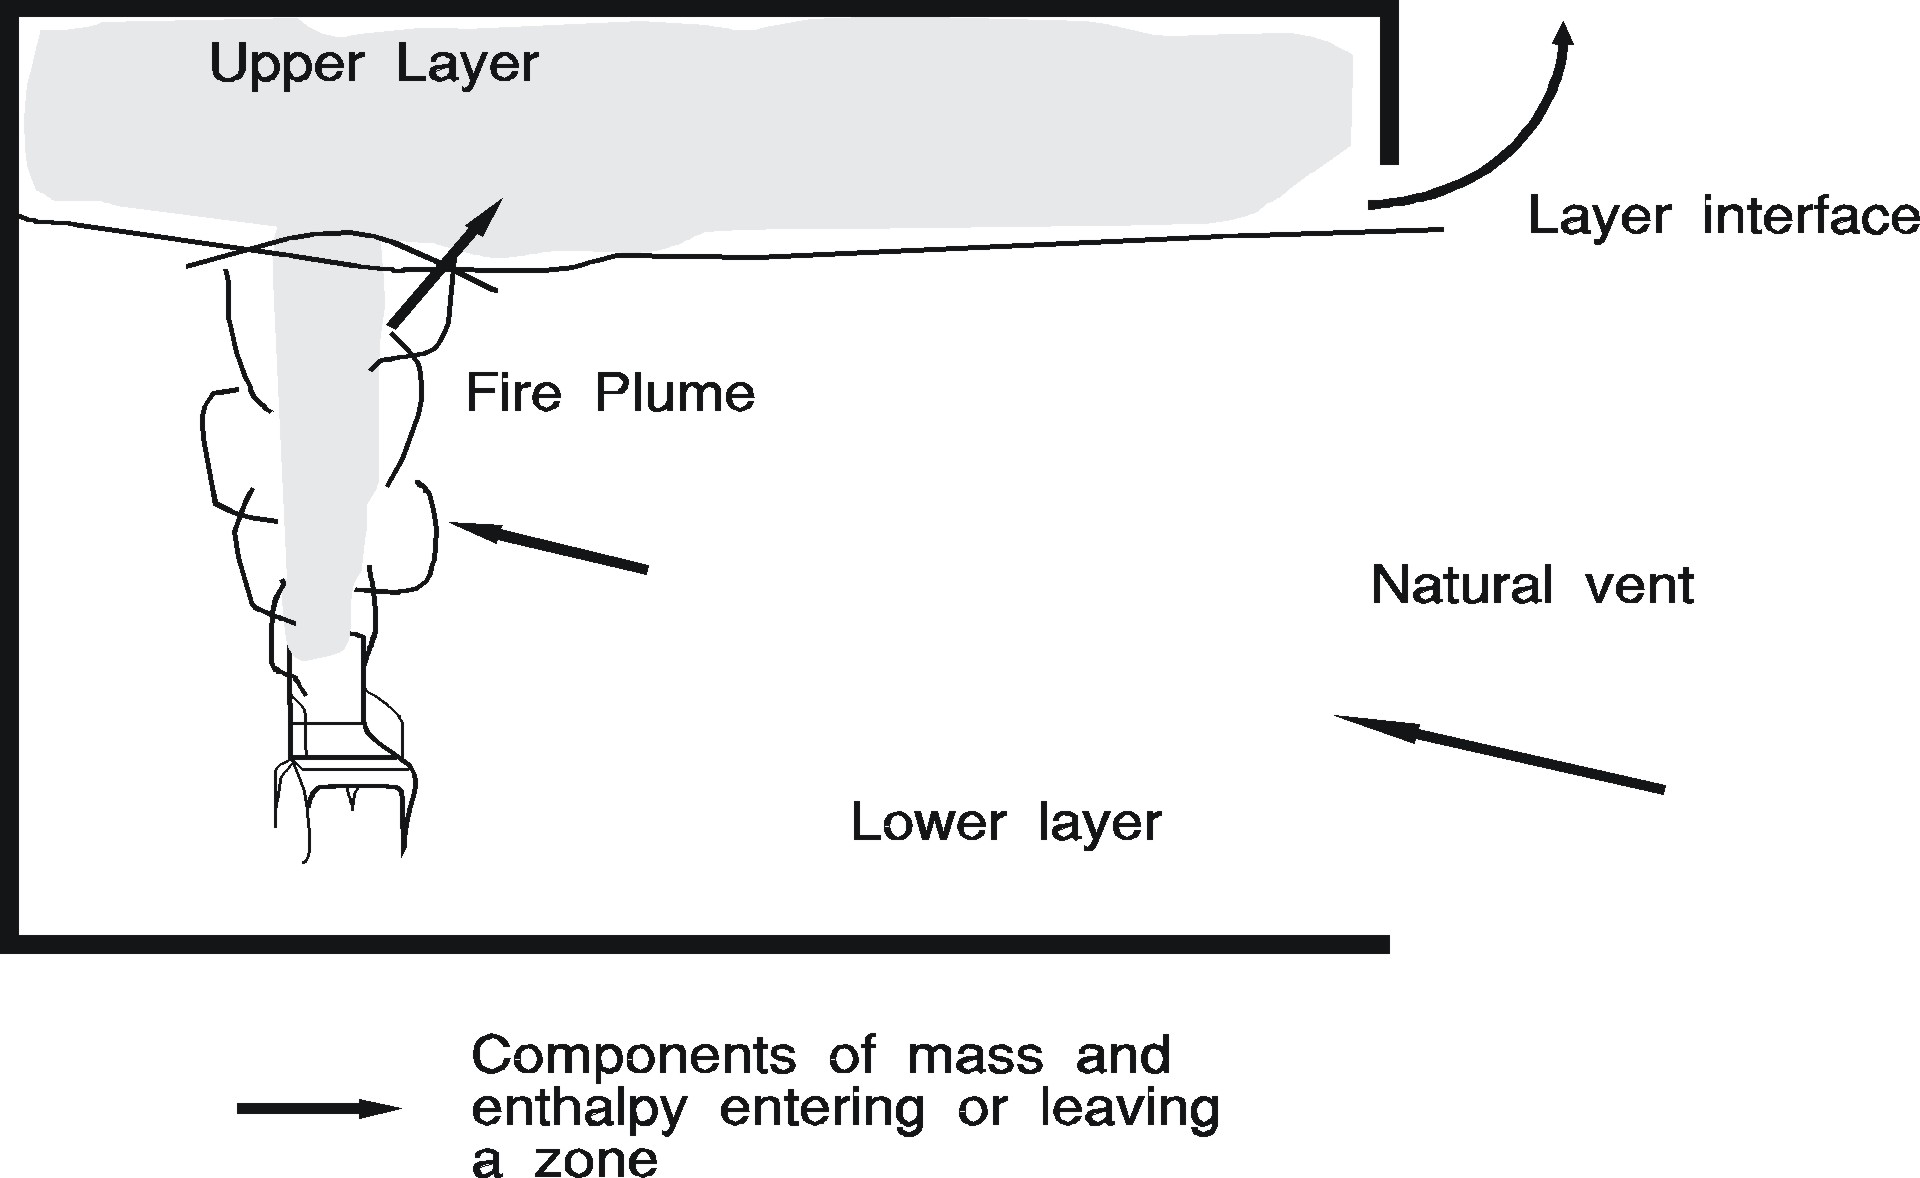
\includegraphics[width=\textwidth]{FIGURES/Theory/Control_Volumes}\\
\end{center}
\caption{Schematic of control volumes in a two-layer zone model.}
 \label{fig:Control_Volumes}
\end{figure}
Conservation of mass in each layer, $\dot m_i$, is expressed
\be
   \dbydt{m_i} = \dot m_i  \label{mass_con}
\ee
Conservation of energy takes the form of the first law of thermodynamics, which states that the rate of increase of internal energy plus the rate at which the layer does work by expansion is equal to the rate at which enthalpy is added to the gas:
\be
   \dbydt{(c_v m_i T_i)} +  P \dbydt{V_i} =  \dot h_i \label{eq:first_law}
\ee
The enthalpy source term, $\dot h_i$, consists of the fire's heat release rate, conduction losses to walls, and radiation exchange. The layer temperature and mass are related to the layer volume and compartment pressure via the ideal gas law:
\be
  P \, V_i = m_i \, R \, T_i \label{EoS}
\ee
A system of ordinary differential equations for the compartment pressure, upper layer volume, and layer temperatures can be derived from these three basic principles:
\begin{eqnarray}
\dbydt{P} &=& \frac{{\gamma-1}}{{V}} \left( \dhl + \dhu \right)  \\[.1in]
\dbydt{\Vu} &=& \frac{1}{P \gamma} \left( (\gamma-1) \, \dhu - \Vu \dbydt{P} \right) \\[.1in]
\dbydt{\Tu} &=& \frac{1}{c_p \, m_{\rm u}} \left( \dhu - c_p \, \dmau \, \Tu + \Vu \dbydt{P} \right) \\[.1in]
\dbydt{\Tl} &=& \frac{1}{c_p \, m_{\rm l}} \left( \dhl - c_p \, \dmau \, \Tl + \Vl \dbydt{P} \right)
\end{eqnarray}
As discussed in Refs.~\cite{Forney:1994} and \cite{Rehm:1992}, these equations are stiff, meaning that the pressure adjusts to changing conditions more quickly than the other variables. Runge-Kutta methods or predictor-corrector methods such as Adams-Bashforth require prohibitively small time steps in order to track the short time scale phenomena (pressure in our case). Methods that calculate the Jacobian (or at least approximate it) have a much larger stability region for stiff problems and are thus more successful at their solution.





\chapter{The Fire Plume}
\label{sec:TheFire}

Fires in CFAST are specified by the user in terms of a time-dependent heat release rate (HRR), an effective fuel molecule, and the yields of the products of incomplete combustion like soot and CO. Fires can be specified in multiple compartments and are treated as totally separate entities, with no interaction of the plumes. These fires are generally referred to as ``objects'' and can be ignited at a prescribed time, temperature or heat flux.

CFAST does not include a pyrolysis model to {\em predict}, as opposed to specify, the growth and spread of the fire. Rather, pyrolysis rates for each fire are prescribed by the user. While this approach does not directly account for increased pyrolysis due to radiative feedback from the flame or compartment, in theory these effects could be prescribed by the user. In an actual fire, this is an important consideration, and the specification used should consider the experimental conditions as closely as possible.

\section{Combustion Chemistry}

 The HRR of the fire is specified by the user, but it may be constrained by the availability of oxygen in the compartment. The combustion of a hydrocarbon fuel is described by the following single-step reaction:
\begin{eqnarray}
   \mathrm{C_{n_\C}H_{n_H}O_{n_O}N_{n_N}Cl_{n_{Cl}}} &+&  \nu_\OTWO \, \mathrm{O_2}  \rightarrow  \nonumber \\[.1in]
   \nu_\COTWO \, \mathrm{CO_2} &+& \nu_\HTWOO \, \mathrm{H_2O} \; + \; \nu_\CO \, \mathrm{CO} \; + \; \nu_\So \, \mathrm{Soot} \; + \; \nu_\HCl \mathrm{HCl} \; + \; \nu_\HCN \mathrm{HCN} \label{stoich}
\end{eqnarray}
The user specifies the composition of the fuel molecule and the yields of soot and CO, $y_\So$ and $y_\CO$, which are related to their stoichiometric coefficients as follows:
\begin{eqnarray}
   \nu_\So &=& \frac{M_\F}{M_\So} \; y_\So \label{soot_yield} \\[.1in]
   \nu_\CO &=& \frac{M_\F}{M_\CO} \; y_\CO \label{CO_yield}
\end{eqnarray}
Under the assumption that all of the nitrogen and chlorine in the fuel are converted to HCN and HCl, the other stoichiometric coefficients are:
\begin{eqnarray}
  \nu_\COTWO &=& \mathrm{n_\C} - \brackets{\nu_\CO + \nu_\HCN + \nu_\So} \\[.1in]
  \nu_\HTWOO &=& \frac{\mathrm{n_\Hy} - \brackets{\nu_\HCl + \nu_\HCN}}{2} \\[.1in]
  \nu_\OTWO  &=& \nu_\COTWO + \frac{\nu_\HTWOO + \nu_\CO - \mathrm{n_\Oh}}{2} \label{Oxygen_yield} \\[.1in]
  \nu_\HCl   &=& \mathrm{n_{Cl}} \\[.1in]
  \nu_\HCN   &=& \mathrm{n_{N}}
\end{eqnarray}
Note that the nitrogen in the air acts only as a diluent. The yields of hydrogen cyanide and hydrogen chloride are based solely on the composition of the fuel molecule. Finally, a user-specified trace species can be specified to follow the transport that results from fire-induced flow for an arbitrary species. This may be of particular interest for radiological releases \cite{Jones:2008}, but may be useful for any trace amounts released by a fire.

\section{Heat Release Rate}
\label{section:HRR}

As fuel and oxygen are consumed, heat is released and various products of combustion are formed. The heat is released as radiation and convected enthalpy:
\begin{eqnarray}
   \dQr &=& \chi_{\rm r} \, \dQ \\[.1in]
   \dQc &=& (1-\chi_{\rm r}) \, \dQ
\end{eqnarray}
where, $\chi_{\rm r}$ is the fraction  of the fire's heat release rate given off as radiation. The default value to 0.30~\cite{Drysdale:1985}.

While it is convenient for the user to directly specify the heat release rate of the fire, it is actually the pyrolysis rate of fuel, $\dmf$, that is specified:
\be
   \dmf = \frac{\dQ}{\Dh}
\ee
where $\Dh$ is the heat of combustion. In the event that the HRR is constrained by the availability of oxygen, the pyrolysis rate does not change, but the HRR becomes:
\be
   \dQ = \min \Big( \dmf \, \Dh \, , \, \dme \, Y_\OTWO \, C_{\rm LOL} \, \DhO \Big)
\ee
where $\dme$ is the entrainment rate, $Y_\OTWO$ is the mass fraction of oxygen in the layer containing the fire, $\DhO$ is the heat of combustion based on oxygen consumption\footnote{The heat of combustion based on oxygen consumption is taken to be 13.1~MJ/kg, representative of typical hydrocarbon fuels~\cite{Huggett:1980}.}, and $C_{\rm LOL}$ is the smoothing function ranging from 0 to 1:
\be
   C_{\rm LOL} = \frac{\tanh \Big( 800 (Y_\OTWO - Y_{\OTWO,{\rm l}}) - 4 \Big) + 1}{2}
\ee
The limiting oxygen mass fraction, $Y_{\OTWO,{\rm l}}$, is 0.1, by default.



\section{Plume Entrainment}

The plume mass entrainment, $\dme(z)$, at a height $z$ above the base of the fire is estimated using Heskestad's correlation~\cite{Heskestad:2002}:
\be
   \dme(z) = 0.196 \, \left( \frac{g \, \rho_\infty^2}{c_p \, T_\infty} \right)^{1/3} \, \dQ_{\rm c}^{1/3} \; \brackets{z - z_0}^{5/3} \;
   \left( 1 + \frac{2.9 \, \dQ_{\rm c}^{2/3}}{ \left( \sqrt{g} \, c_p \, \rho_\infty \, T_\infty \right)^{2/3} \, (z-z_0)^{5/3}} \right) \label{mdot_e}
\ee
where $z_0$ is a virtual origin defined as
\be
   \frac{z_0}{D} = -1.02 + 1.4 \, \dQ^{* \, 2/5} \quad ; \quad \dQ^* = \frac{\dQ}{\rho_\infty \, c_p \, T_\infty \, \sqrt{g \, D} \, D^2} \label{virtual_origin}
\ee
Note that the virtual origin is defined in terms of the total heat release rate of the fire, $\dQ$. Equation~(\ref{mdot_e}) is recommended above the mean flame height, $L$. Below the flame height, Heskestad recommends the following:
\be
  \dme(z) = \dme(L) \, \frac{z}{L} \quad ; \quad \frac{L}{D} = -1.02 + 3.7 \, \dQ^{* \, 2/5}
\ee
The mean flame height is defined as the distance from the fuel source to the top of the visible flame where the intermittency is 0.5.  A flame intermittency of 0.5 means that the visible flame is above the mean 50~\% of the time and below the mean 50~\% of the time.

In CFAST, there is a constraint on the mass entrainment rate because the plume can rise only so high for a given HRR.  Early in a fire, the plume may not have sufficient energy to reach the compartment ceiling. Therefore, a limit is placed on the entrainment rate. For the plume to be able to penetrate the hot upper layer, the density of the gas in the plume must be less than the density of the gas in the upper layer. This implies that the upper layer temperature must be less than the plume temperature:
\be
   \Tu < \Tp \approx \frac{ \dQc + \dme \, c_p \, \Tl }{ \dme \, c_p}
\ee
Rearranging terms yields a limit on the mass entrainment:
\be
   \dm_e < \frac{\dQc}{c_p (\Tu - \Tl)}
\ee


\section{Plume Centerline Temperature}

The centerline plume temperature rise, $\Delta T_0(z)$, at a height $z$ above the base of the fire is estimated using Heskestad's correlation~\cite{Heskestad:2002}:
\be
   \Delta T_0(z) = 9.1 \, \left( \frac{T_\infty}{g \, c_p^2 \, \rho_\infty^2} \right)^{1/3} \, \dQ_{\rm c}^{2/3} \, (z-z_0)^{-5/3}  \label{plume_temperature}
\ee
where the virtual origin, $z_0$, is defined in Eq.~(\ref{virtual_origin}). Equation~(\ref{plume_temperature}) is valid above the flame height, $L$, and below the hot gas layer interface, $z_{\rm I}$. Below the flame height, the temperature rise is approximated at 900~K. Above the layer interface, the temperature and density of the entrained air is significantly different than that of the lower layer. To account for this, the temperature correlation is modified for values of $z$ greater than the interface height, $z_{\rm I}$:
\be
   \Delta T_0(z) = 9.1 \, \left( \frac{\Tu}{g \, c_p^2 \, \rho_{\rm u}^2} \right)^{1/3} \, \dQ_{\rm c}^{2/3} \, (z-z_0')^{-5/3}  \quad ; \quad z>z_{\rm I}  \label{plume_temperature_upper}
\ee
where the modified virtual origin is given by:
\be
   z_0' = z_{\rm I} - \left( \frac{\Tu}{\Tl} \right)^{3/5} \, (z_{\rm I}-z_0)  \label{virtual_origin_modified}
\ee
Equations~(\ref{plume_temperature_upper}) and (\ref{virtual_origin_modified}) are obtained by asserting that $\Delta T_0$ is continuous across the layer interface and that $\Tu \rho_{\rm u} \approx \Tl \rho_{\rm l}$.

The mass entrainment correlation, Eq.~(\ref{mdot_e}), is modified the same way above the layer interface.



\chapter{Ventilation}

CFAST models three types of vent flow: natural flow through vertical vents (such as doors or windows),  natural flow through horizontal vents (such as ceiling holes or hatches), and forced flow via mechanical ventilation. Forced flow can occur through either vertical or horizontal vents.

Atmospheric pressure is about 100~kPa. Fires produce pressure changes from 1~Pa to 1~kPa and mechanical ventilation systems typically involve pressure differentials of about 1~Pa to 100~Pa.  The pressure variables are solved to a higher accuracy than other solution variables because of the subtraction (with resulting loss of precision) needed to calculate vent flows from pressure differences.


\section{Vertically-Oriented Vents (Doors and Windows)}

Natural flow through windows and doors is governed by the pressure difference across the opening.  A momentum equation for the zone boundaries is not solved directly.  Instead momentum transfer at the zone boundaries is included by using Bernoulli's equation augmented for restricted openings with an orifice coefficient~\cite{Quintiere:1984, Steckler_Coefficients}.

The mass flow through a vertical opening is calculated by dividing the vertical extent of the opening into discrete segments, each of which is bounded by either the top or bottom of the door or window, the zone interface of either compartment, or the neutral plane, which is where the velocity changes direction. In this way, the vent opening is partitioned into at most six sections.

Let $z=b$ and $z=t$ denote the height of the bottom and top of the segment, and $\Delta P_b$ and $\Delta P_t$ denote the pressure differences at those heights.  Because the segment is either completely above or completely below the neutral plane, the two pressure differences will have the same sign. The mass flow through the segment can then be computed by integrating from $b$ to $t$:
\begin{eqnarray}
\dm &=& \int_b^t C \sqrt{2 \rho \, \Delta P(z)} \, w \, dz  \\[.1in]
    &=& C\sqrt{2\rho} \, w \int_b^t\sqrt{\frac{|(t-z) \, \Delta P_b + (z-b) \, \Delta P_t|}{t-b}} \; dz \\[.1in]
    &=& \frac{2}{3} \, C \sqrt{2\rho} \, w \, (t-b)\frac{|\Delta P_t|^{3/2}-|\Delta P_b|^{3/2}}{|\Delta P_t|-|\Delta P_b|}
\label{eq:massflowone}
\end{eqnarray}
Here, $C$ is the orifice coefficient taken to be 0.7~\cite{Steckler_Coefficients}, $\rho$ is the gas density of the upwind compartment, and $\Delta P(z)$ is the pressure across the interface at elevation $z$. Note that the integral is evaluated from
\begin{eqnarray}
\int \sqrt{A+Bz} \, dz = \frac{2}{3B}(A+Bz)^{3/2}+\mbox{constant}
\end{eqnarray}
where $A=(|t\,\Delta P_t|-b\,|\Delta P_b|)/(t-b)$ and $B=(|\Delta P_t|-|\Delta P_b|)/(t-b)$.
Equation \ref{eq:massflowone} is sometimes written:
\be
   \dm = \frac{2}{3} C \sqrt{2 \rho} \, w \, (t-b)  \frac{|\Delta P_t|+\sqrt{|\Delta P_t \,\Delta P_b|}+|\Delta P_b|}{\sqrt{|\Delta P_t|}+\sqrt{|\Delta P_b|} }
\ee
The mass flows through the various vertical segments of the door or window are distributed into the upper and lower layers of the downstream compartment depending on the temperature of the stream. Consider the flow of gas from the upper layer of Compartment~1 entering the lower layer of Compartment~2 (see Fig.~\ref{fig:Flow_Patterns}).
\begin{figure}[t]
\setlength{\unitlength}{1in}
\begin{picture}(6.5,4)
\thicklines
\put(0,0){\line(1,0){6.5}}
\put(0,4){\line(1,0){6.5}}
\put(3.25,4){\line(0,-1){1}}
\thinlines
\put(0,1.5){\line(1,0){3.25}}
\put(3.25,2.5){\line(1,0){3.25}}
\put(0,2.0){\line(1,0){6.5}}
\put(3.5,0.75){\vector(-1,0){0.5}}
\put(3.5,1.75){\vector(-1,0){0.5}}
\put(3,2.25){\vector(1,0){0.5}}
\put(3,2.75){\vector(1,0){0.5}}

\put(1.625,3.8){\makebox(0,0){Compartment 1}}
\put(4.875,3.8){\makebox(0,0){Compartment 2}}
\put(6,1.85){\makebox(0,0){Neutral Plane}}
\put(5.95,2.35){\makebox(0,0){Layer Interface}}
\put(0,1.35){Layer Interface}
\put(3.75,0.75){\makebox(0,0){$\dm_{\rm l \to l}$}}
\put(3.75,1.75){\makebox(0,0){$\dm_{\rm l \to u}$}}
\put(2.75,2.25){\makebox(0,0){$\dm_{\rm u \to l}$}}
\put(2.75,2.75){\makebox(0,0){$\dm_{\rm u \to u}$}}

\end{picture}
\caption{Flow patterns for horizontal flow through a vertical vent.}
\label{fig:Flow_Patterns}
\end{figure}
The mass flow rate is denoted $\dm_{\rm u \to l}$, where the subscripts indicate the upstream and downstream layer indices, respectively. The enthalpy flow rate is:
\be
   \doh_{\rm u \to l} = c_p \brackets{T_{\rm u,1}-T_{\rm l,2}} \, \dm_{\rm u \to l}
\ee
Assuming that $T_{\rm l,2} < T_{\rm u,1} < T_{\rm u,2}$, this energy will be distributed between the compartment's two layers. The distribution is based on the relative difference in temperature between the incoming gas stream and the layer temperatures. Some of the energy stays within the lower layer and some of the energy goes to the upper layer in the form of a virtual plume. The effective heat release rate of this virtual plume is:
\be
   \dQ_{\rm eff} = \frac{T_{\rm u,1}-T_{\rm l,2}}{T_{\rm u,2}-T_{\rm l,2}} \; \doh_{\rm u \to l}
\ee
The mass entrainment rate into this virtual plume at the midpoint of the vertical segment, $\bar{z}$, is assumed to be a fraction of the incoming mass flow rate:
\be
   \dm_{\rm e,eff} = \frac{T_{\rm u,1}-T_{\rm l,2}}{T_{\rm u,2}-T_{\rm l,2}} \; \dm_{\rm u \to l}
\ee
The origin of the virtual plume, $z_0$, is deduced from the plume mass entrainment correlation, Eq.~\ref{mdot_e}. That is, $z_0$ is the origin of the virtual plume whose convective heat release rate is $\dQ_{\rm eff}$ and whose mass entrainment rate is $\dm_{\rm e,eff}$ at the midpoint of the segment, $\bar{z}$:
\be
   z_0 = \bar{z} - \dm_{\rm e,eff}^{3/5} \, \left[ 0.196 \, \left( \frac{g \, \rho_\infty^2}{c_p \, T_\infty} \right)^{1/3} \, \dQ_{\rm eff}^{1/3} \right]^{-3/5}
\ee

The other type of mixing is much like an inverse plume and causes contamination of the lower layer.  It occurs when there is flow of the type $\dm_{42} > 0$.  The shear flow causes vortex shedding into the lower layer and thus some of the particulates end up in the lower layer.  The actual amount of mass or energy transferred is usually not large, but its effect can be large.  For example, even minute amounts of carbon can change the radiative properties of the gas layer, from negligible to something finite.  It changes the rate of radiation absorption significantly and invalidates the simplification of an ambient temperature lower layer.  This term is predicated on the Kelvin-Helmholz flow instability and requires shear flow between two separate fluids.  The mixing is enhanced for greater density differences between the two layers. However, the amount of mixing has never been well characterized. Quintiere et al. \cite{Quintiere:1984} discuss this phenomena for the case of crib fires in a single room, but their correlation does not yield good agreement with experimental data in the general case \cite{Quintiere:1981}.  In the CFAST model, it is assumed that the incoming cold plume behaves like the inverse of the usual door jet between adjacent hot layers; thus we have a descending plume.  The same equations are used to calculate this inverse plume as are used for the upright door mixing, above. It is possible that the entrainment is overestimated in this case, since buoyancy, which is the driving force, is not nearly as strong as for the usually upright plume.

\section{Horizontally-Oriented Vents (Floor and Ceiling Vents)}

Flow through a ceiling or floor vent is governed by both pressure and density differences. The simplest form is uni-directional flow driven primarily by a relatively large pressure difference. When the pressure difference is relatively small, the density difference, where hot gas underlies colder gas, can lead to bi-directional flow where the gas in the lower compartment rises into the upper compartment and {\em vice versa}.  This situation might arise in a real fire if the room of origin suddenly has a hole open up in the ceiling.

Cooper's algorithm~\cite{Cooper:1989, Cooper:1990, Cooper:1995} is used for computing mass flow through ceiling and floor vents:
\be
   \dm = 0.1 \brackets{\frac{g \, \Delta \rho \, A_{\rm v}^{5/2}}{\rho_{\rm avg}}} \brackets{1 - \frac{2 \, A_{\rm v}^2 \, \Delta P}{S^2 \, g \, \Delta \rho \, D^5}}
\ee
where $D = 2 \sqrt{A_{\rm v} / \pi}$ and $S$ is 0.754 for round or 0.942 for square openings, respectively. For each layer on either side of the vent, there are two values of the mass flow, $\dm_{\rm in}$ and $\dm_{\rm out}$. These terms are symmetric: the outgoing flow from one compartment is the incoming flow to the other. The corresponding enthalpy flows are determined from the relative size and temperature of the lower and upper layers:
\begin{eqnarray}
  \doh_{\rm in} &=& c_p \, \dmu \, \Tu + c_p \, \dml \, \Tl \\[0.1in]
  \dmu &=& \dm_{\rm in} \, \frac{\Vu}{V} \\[0.1in]
  \dml &=& \dm_{\rm in} \, \frac{\Vl}{V}
\end{eqnarray}
The mass and energy are then deposited into the upper or lower layer of the receiving compartment based on the effective temperature of the incoming flow relative to the upper and lower layers of the receiving compartment. If the temperature of the incoming flow is higher than the temperature of the lower layer, then the flow is deposited into the upper layer. This is similar to the idea of using a virtual plume for a doorway flow.


\section{Forced Flow}

CFAST models mechanical ventilation in terms of user-specified volume flows at various points in the compartment. The model does not include duct work or fan curves. These equations are high-order, non-linear and in some cases ill-posed, which caused a great deal of difficulty in reaching a numerical solution.

Figure~\ref{fig:Fans_and_Ducts}(a) depicts smoke exhaust via a fan at the top of an atrium, and Fig.~\ref{fig:Fans_and_Ducts}(b) illustrates a kitchen exhaust fan.  Cross ventilation, shown in Fig.~\ref{fig:Fans_and_Ducts}(c), is occasionally used without heating or cooling.  Generally systems that maintain comfort conditions have either one or two fans. Further information about these systems is presented in Klote and Milke~\cite{Klote:2002} and the American Society of Heating, Refrigerating and Air Conditioning Engineers (ASHRAE) \cite{ASHRAE:2001}.

\begin{figure}
\begin{center}
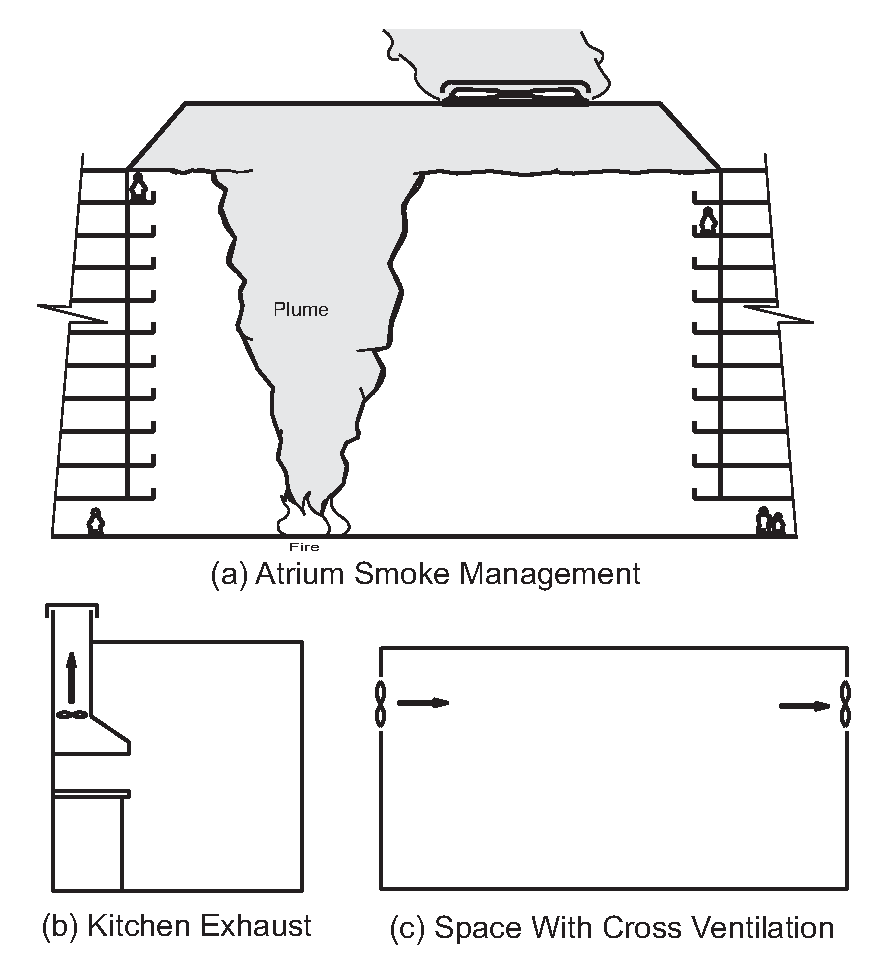
\includegraphics[width=5.0in]{FIGURES/Theory/HVAC_Fans_and_Ducts}\\
\end{center}
\caption{Some simple fan-duct systems.}
 \label{fig:Fans_and_Ducts}
\end{figure}

The flow through mechanical vents can be filtered. Filtering affects particulates such as smoke and the trace species. Filtering can be turned on at any time. Effectiveness is from 0~\% (no effect) to 100~\% which completely blocks flow of these two species.





\chapter{Heat Transfer}

This section discusses thermal radiation, convection and conduction, the three mechanisms by which heat is transferred between the gas layers and the enclosing compartment walls. Hot gases exchange heat with solid surfaces via convection and radiation. Heat is transferred through solids via conduction. Different material properties can be used for the ceiling, floor, and walls of each compartment (although all the walls of a compartment must be the same).  Additionally, each surface can be composed of up to three distinct layers.  This allows the user to deal naturally with the actual building construction.  Material thermophysical properties are assumed to be constant. Radiative transfer occurs among the fire(s), gas layers and compartment surfaces (ceiling, walls and floor).  This transfer is a function of the temperature differences and the emissivity of the gas layers as well as the compartment surfaces.  Typical surface emissivity values only vary over a small range.  For the gas layers, however, the emissivity is a function of the concentration of species which are strong radiators, predominately smoke particulates, carbon dioxide, and water.

\section{Radiation}
\label{sec:Radiation}

Radiation heat transfer is calculated between the ceiling, floor, wall layers, and fire, with the inclusion of emission and absorption by the hot gas layer~\cite{Forney_radiation}. The following assumptions are made:
\begin{itemize}
\item Each gas layer and each wall segment is assumed to be at a uniform temperature.
\item The wall and gas layer temperatures are assumed to change slowly over the duration of the time step of the governing equations.
\item The fire is assumed to radiate uniformly in all directions emitting a fraction, $\chi_{\rm r}$, of the total heat release rate.  This radiation is assumed to originate from a single point.  Radiation feedback to the fire and radiation from the plume is not modeled in the radiation exchange algorithm.
\item The radiation emitted is assumed to be diffuse and gray.  In other words, the radiant fluxes emitted are independent of direction and wavelength. At a solid surface, the emittance, $\epsilon$, absorptance, $\alpha$ and reflectance, $\rho$, are related via $\epsilon = \alpha = 1 - \rho$. In the gas phase, the emittance, $\epsilon$, absorptance, $\alpha$ and transmittance, $\tau$, are related via $\epsilon = \alpha = 1 - \tau$.
\item Rooms or compartments are assumed to be rectangular boxes.  Each wall is either perpendicular or parallel to every other wall.  Radiation transfer through vent openings is lost from the room.
\end{itemize}
The compartment lining is divided into four parts: the ceiling, the floor, and the wall sections above and below the layer interface. The net radiative heat flux at surface~$k$, $\dq_k''$, is found by solving the simplified radiation transport equation given by Eq.~(17-20) in Siegel and Howell~\cite{SiegelandHowell:1981}:
\be
   \frac{\dq_k''}{\epsilon_k} - \displaystyle\sum_{j=1}^N \frac{1 - \epsilon_j}{\epsilon_j} \, \dq_j'' \, F_{k-j} \, \tau_{k-j} = \sigma T_k^4 - \displaystyle\sum_{j=1}^N \brackets{\sigma T_j^4 \, F_{k-j} \, \tau_{k-j}} - c_k \label{RTE}
\ee
where $F_{k-j}$ is the configuration factor (fraction of radiant energy emitted by surface $j$ that is intercepted by surface $k$), $\tau_{k-j}$ is the transmittance, $\sigma$ is the Stefan-Boltzman constant, $\epsilon_k$ is the emissivity, $A_k$ is the area, and $T_k$ is the temperature of surface $k$. The radiation from the hot gas layer and the fire is included in the last term:
\be
   c_k = \epsilon_{\rm u} \, F_{{\rm u}-k} \, \sigma \, \Tu^4 + \frac{\omega_{{\rm f}-k}}{4 \pi} \frac{\chi_{\rm r} \, \dQ}{A_k}  \label{ckeq}
\ee
where $\epsilon_{\rm u}$ is the emittance (absorptance) of the upper layer, $F_{{\rm u}-k}$ is the view factor between the upper layer and solid surface, $\omega_{{\rm f}-k}$ is the solid angle between the fire and wall\footnote{Note that as the area of surface $k$ shrinks to zero, $\omega_{{\rm f}-k}/A_k \to 1/R^2$, yielding the classic point source radiation model}, and $\dQ$ is the heat release rate of the fire. If the solid surface, $k$, is the floor or the lower wall, the view factor refers to the layer interface. If the solid surface, is the upper wall or ceiling, the view factor is 1.

Reference~\cite{Forney_radiation} describes the solution of Eq.~\ref{RTE}.


\subsubsection{Configuration Factors}

The configuration factor, $F_{1-2}$, is the fraction of radiant energy emitted by surface 1 that is intercepted by  surface 2, and is calculated:
\be
   F_{1-2} = \frac{1}{A_1} \int_{A_1} \int_{A_2} \frac{\cos \theta_1 \, \cos \theta_2}{\pi L^2} \, dA_2 \, dA_1 \label{eq:config_factor}
\ee
where $L$ is the distance along the line of integration,  $\theta_1$ and $\theta_2$ are the angles for surface 1 and 2 between the respective normal vectors and the line of integration, and $A_1$ and $A_2$ are the areas of the two surfaces.  These terms are illustrated in Fig.~\ref{fig:Rad_Config_Factor}.  
\begin{figure}
\begin{center}
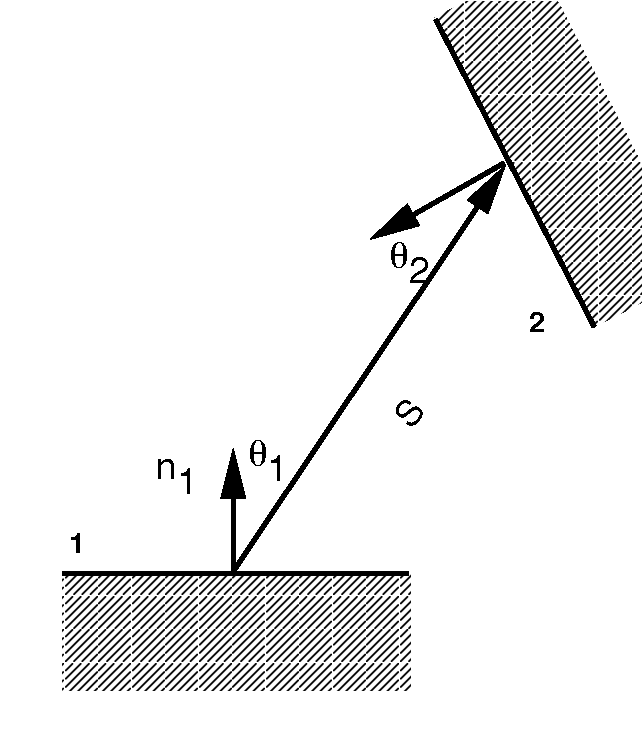
\includegraphics[width=3.0in]{FIGURES/Theory/Radiation_Config_Factor}\\
\end{center}
\caption{Setup for a configuration factor calculation between two arbitrarily oriented finite areas.}
 \label{fig:Rad_Config_Factor}
\end{figure}
There are two types of configuration factors in CFAST. First, consider two rectangles perpendicular to each other having a common edge of the same length, $l$. The dimension of the source rectangle is $l \times w$ and the target rectangle is $l \times h$. The configuration factor from source to target is:
\begin{eqnarray}
\lefteqn{F_{1-2} = \frac{1}{\pi \, W} \left[ W \, \tan^{-1} \frac{1}{W} + H \, \tan^{-1} \frac{1}{H} - \sqrt{H^2+W^2} \, \tan^{-1} \frac{1}{\sqrt{H^2+W^2}} + \right.}  \nonumber \\[.1in]
& &   \left. \frac{1}{4} \, \ln \left\{ \frac{(1+W^2)(1+H^2)}{1+W^2+H^2} \, \left( \frac{W^2(1+W^2+H^2)}{(1+W^2)(W^2+H^2)} \right)^{W^2} \left( \frac{H^2(1+W^2+H^2)}{(1+H^2)(W^2+H^2)} \right)^{H^2} \right\} \right]
\end{eqnarray}
where $H=h/l$ and $W=w/l$. 

Next, consider two identical, parallel, directly opposed rectangles. The dimension of the rectangles is $a \times b$ and the separation distance is $c$. The configuration factor is:
\begin{eqnarray}
\lefteqn{F_{1-2} = \frac{2}{\pi \, X \, Y} \left\{ \ln \left[ \frac{(1+X^2)(1+Y^2)}{1+X^2+Y^2} \right]^{1/2} + X \sqrt{1+Y^2} \, \tan^{-1} \frac{X}{\sqrt{1+Y^2}} + \right.} \nonumber \\[.1in]
& & \left. Y \sqrt{1+X^2} \, \tan^{-1} \frac{Y}{\sqrt{1+X^2}} - X \, \tan^{-1} X - Y\, \tan^{-1} Y \right\}
\end{eqnarray}
where $X=a/c$ and $Y=b/c$. These formulae are found in Appendix~C of Ref.~\cite{SiegelandHowell:1981}.

Next, the normalized solid angle, $\omega_{\rm f-k}$, in Eq.~(\ref{ckeq}) is computed. First, place a sphere of radius, $r$ tangent to a rectangle of dimension $x \times y$ such that the point of tangency is the corner of the rectangle. The normalized solid angle formed by the center of the sphere and the edges of the rectangle is given by: 
\be
   \omega(x,y;r) = \frac{1}{4\pi} \left[ \sin^{-1} \left( \frac{A \, y}{\sqrt{y^2+r^2}} \right) + \sin^{-1} \left( \frac{A \, x}{\sqrt{x^2+r^2}} \right) - \frac{\pi}{2} \right] \quad ; \quad A=\sqrt{1+\frac{r^2}{x^2+y^2}}
\ee
Suppose now that the radiation of a fire is assumed to emanate from a point a distance $r$ above the floor whose dimension is $L \times W$. Suppose also that the floor is divided into four quadrants based on the location of the fire. The dimensions are partitioned $L=L_1+L_2$ and $W=W_1+W_2$. The normalized solid angle between the point source fire, f, and the floor, fl, is: 
\be
   \omega_{\rm f-fl} = \sum_{j=1}^2 \sum_{i=1}^2 \omega(L_i,W_j;r)
\ee

\subsubsection{Transmittance and Absorptance}

The transmittance is the fraction of radiant energy that will pass through a volume filled with an absorbing media. It is usually expressed in the form:
\be
   \tau = {\rm e}^{-a L}
\ee
where $a$ is the absorption coefficient and $L$ is the path length. The absorptance is the fraction of radiant energy absorbed by that volume. For a gray gas, $\alpha + \tau = 1$.

In general, the transmittance and absorptance are functions of wavelength. This is an important factor to consider for the major gaseous products, $\textnormal{CO}_2$  and $\textnormal{H}_2 \textnormal{O}$. However soot has a continuous absorption spectrum that allows the transmittance and absorptance to be approximated as ``gray'' \cite{SiegelandHowell:1981} across the entire spectrum. The total transmittance over a path length $L$ through a volume of combustion products is taken as the product of the transmittance of the soot and major product gases:
\be
   \tau = e^{-a_{\rm s}L} \brackets{1 - \alpha_{\rm H_2O} - 0.5 \, \alpha_{\rm CO_2}}
\ee
The factor of 0.5 applied to the absorptance of CO$_2$ accounts for the overlap of the wavelength bands of the two gases. Tien~et~al.~\cite{Tien:2002} suggest that the absorption coefficient for soot may be approximated $a_{\rm s} = k f_v T$ where $k$ is a constant that depends on the optical properties of the soot particles, $f_v$ is the soot volume fraction, and $T$ is the (absolute) temperature. Values of $k$, have been found to be about constant for a wide range of fuels~\cite{Tien:1978}.

Absorptance data for $\textnormal{H}_2 \textnormal{O}$ and $\textnormal{CO}_2$ are reported in Ref.~\cite{Edwards:1985}. For each gas, these data are tabulated in a look-up table, implemented as a two-dimensional array based on temperature and gas concentration.

The effective path length, $L$, for the upper gas layer is approximated to be 1.8 times its depth~\cite{Tien:2002}.




\section{Convection}

The transfer of heat between the gas and solid surfaces is handled slightly differently at the ceiling, floor and walls, due to the difference in orientation and the presence of a relatively thin hot flow near the ceiling known as the ceiling jet. The following two sections describe how the convective heat transfer is done for these different surfaces.

\subsection{Walls and Floor}

In general, the convective heat flux to a solid surface is given by:
\be
   \dqc'' = h \, \brackets{\Tg - \Ts}  \label{convective_heat_flux}
\ee
The convective heat transfer coefficient, $h$, is a function of the gas properties, temperature, and velocity. In CFAST, simple correlations for natural convection are used since the gas velocity is unknown:
\be
   h = C {|\Tg - \Ts|}^{1/3}
\ee
where $C$ is an empirical coefficient (1.52 for the floor and ceiling (in the absence of a ceiling jet) and 1.31 for the walls~\cite{Holman:1990}), $\Tg$ is the average gas layer temperature adjacent to the surface, and $\Ts$ is the surface temperature.

\subsection{Ceiling}

During the early stage of a fire before a hot gas layer has formed, the convective heat transfer to the ceiling is governed by the temperature and velocity of the ceiling jet. Alpert's chapter in the {\em SFPE Handbook}~\cite{Alpert:SFPE} presents an empirical correlation for the convective heat flux from the ceiling jet to a relatively cool surface:
\be
   \dqc'' = 1.323 \, f \, \frac{\dQ_{\rm c}}{H^2} \, \left( \frac{r}{H} \right)^{-1.36}  \label{eq:cjflux}
\ee
where $f$ is a friction factor estimated to be 0.03, $r$ is the radial distance to the plume centerline, $H$ is the ceiling height, and $\dQ_{\rm c}$ is the convective fraction of the heat release rate. The average convective heat flux to the ceiling can be obtained by integrating this expression over the entire ceiling:
\be
   \dq_{\rm c,avg}'' = \frac{1}{LW} \int_0^{2\pi} \int_0^R \dqc'' \, r \, dr \, d\theta = \frac{0.27 \, \dQ_{\rm c}}{(LW)^{0.68} \, H^{0.64}} \label{eq:cjfluxavg}
\ee
Note that the integration is carried out over a circle whose area, $\pi R^2$, is equal to the area of the ceiling, $LW$.

Equation~(\ref{eq:cjfluxavg}) applies to the early stage of the fire; thus, a modified heat transfer coefficient is used so that there is a transition from the early to later stages when a layer has formed:
\be
   h = \max \left( \frac{\dq_{\rm c,avg}''}{\Tu-\Ts} \, , \, C {|\Tu - \Ts|}^{1/3} \right)
\ee
Here, $\Tu$ is the average temperature of the upper layer and $\Ts$ is the ceiling surface temperature. Notice that the rightmost term is simply the correlation used for the walls and floor.

\section{Conduction}

The heat conduction equation is solved in the direction normal to solid target or wall surfaces using non-uniformly spaced nodes and a second order accurate central difference scheme for the spatial derivatives and a semi-implicit time marching scheme. At each time step, the internal solid temperatures are updated in time until the net convective and radiative heat flux striking the wall equals with the heat flux into the solid~\cite{Moss:1992}:
\be
   \dq'' \equiv \dqr'' + \dqc'' = -k \, \frac{dT}{dx} \Big|_{x=0}
\ee
where $k$ is the thermal conductivity of the solid.  This solution strategy requires a differential algebraic equation (DAE) solver that can simultaneously solve both differential and algebraic equations.  With this method, only one or two extra equations are required per wall segment (two if both the interior and exterior wall segment surface temperatures are computed).  This solution strategy is more efficient than the method of lines since fewer equations need to be solved. Conduction is then coupled to the gas phase energy exchange.

A non-uniform array of internal nodes is used to capture steep gradients in temperature near the surface. Define a penetration depth of
\be
   x_p = 2 \sqrt{\alpha \, t_{\rm end}} \; \hbox{erfc}^{-1} \brackets{0.05}
\ee
where $\hbox{erfc}^{-1}$ denotes the inverse of the complementary error function. The value $x_p$ is the location in a semi-infinite wall where the temperature rise is 5~\% after $t_{\rm end}$ seconds. Eighty percent of the nodes are placed on the interior side of $x_p$ and the remaining 20~\% are placed on the exterior side.

The heat conduction equation normal to the solid surface is:
\be \frac{\partial T}{\partial t} = \frac{k}{\rho c}\frac{\partial^2 T}{\partial x^2}
\label{eq:Target_PDE} \ee
where $k$, $\rho$ and $c$ are the thermal conductivity, density and heat capacity of the target. At the surface, $x=0$, the boundary condition is:
\be
   \dq''=-k\frac{dT}{dx} \label{eq:Target_Fourier}
\ee
where $\dq''$ is the net convective and radiative heat flux.

\newcommand{\Dt}{\Delta t}
\newcommand{\Dr}{\Delta r}
\newcommand{\Tipo}{T_{i+1}^{n+1}}
\newcommand{\Ti}{T_{i}^{n+1}}
\newcommand{\Timo}{T_{i-1}^{n+1}}

The 1-D heat conduction equation can be solved in either Cartesian or cylindrical coordinates. The solution methodology shall be presented for cylindrical coordinates:
\be 
  \frac{\partial T}{\partial t} = \frac{k}{\rho c} \frac{1}{r} \frac{\partial}{\partial r} \left( r \frac{\partial T}{\partial r} \right)
\ee
Dividing the cylinder into $N$ uniformly spaced concentric control volumes, this equation can be written in discretized form:
\begin{eqnarray}
\Ti-T_i^n&=& \frac{\Dt}{\Dr} \frac{k}{\rho c}
\left[
\left(\frac{\Tipo-\Ti}{\Dr}\right)
\frac{r_i}{r_{i-1/2}}-
\left(\frac{\Ti-\Timo}{\Dr}\right)
\frac{r_{i-1}}{r_{i-1/2}}
\right]
\nonumber\\[0.2in]
&=&\frac{\Dt \, \alpha}{\Dr^2}
\left[
\left(\Tipo-\Ti\right)
\left(\frac{i}{i-0.5}\right)-
\left(\Ti-\Timo\right)
\left(\frac{i-1}{i-0.5}\right)
\right]
\label{eq:cylheat6}
\end{eqnarray}
where $\alpha=k/(\rho c)$. Defining $C_i$ and $D_i$ as
\be
C_i = \frac{\alpha\Dt}{\Dr^2}\left(\frac{i-1}{i-0.5}\right) \quad ; \quad D_i = \frac{\alpha\Dt}{\Dr^2}\left(\frac{i}{i-0.5}\right)
\ee
Eq.~(\ref{eq:cylheat6}) can be written:
\be
-C_i \, \Timo + \left( 1+2\frac{\alpha\Dt}{\Dr^2} \right) \, \Ti - D_i \, \Tipo = T_i^n  \quad \quad i=1...N-1
\label{eq:cylheat8}
\ee
The boundary condition is applied at control volume $N$:
\begin{eqnarray*}
T_N^{n+1}-T_N^n=\frac{\alpha\Dt}{\Dr^2}
\left[\frac{\Dr \, \dq''}{k} \frac{N}{N-0.5} -(T_N^{n+1}-T_{N-1}^{n+1}) \frac{N-1}{N-0.5} \right]
\end{eqnarray*}
or
\be
-C_N \, T_{N-1}^{n+1}+ \left( 1+C_N \right) T_N^{n+1} = T_N^n+D_N\frac{\Dr}{k} \dq''
\label{eq:cylheat10}
\ee
The internal temperature profile, $T_i$, is then obtained with a tri-diagonal linear solver.




\section{Coupling the Gas and Solid Phase Calculations}

To illustrate the method, consider a one room case with one active wall.  There are four gas phase equations (pressure, upper layer volume, upper and lower layer temperatures) and one wall temperature equation.  Implementation of the gradient matching method requires that storage be allocated for the temperature profiles at the current time step, $t$, and at the next time step, $t + \Delta t$.  Given the profile at time $t$ and values for the five unknowns at time $t + \Delta t$ (initial guess by the solver), the temperature profile is advanced from time $t$ to $t + \Delta t$.  The temperature gradient at the wall surface is computed followed by the residuals for the five equations.  The DAE solver adjusts the solution variables and the time step until the residuals for all the equations are below an error tolerance.  Once the solver has completed the step, the array storing the temperature profile for the previous time is updated, and the DAE solver is ready to take its next step.

Heat transfer between connected compartments is modeled by merging the back surfaces of the connected ceiling and floor of the compartments or the back wall surfaces of the connected horizontal compartments.  A heat conduction problem is solved for the merged walls using a temperature boundary condition for both the near and far wall.  As before, temperatures are determined by the DAE solver so that the heat flux striking the wall surface (both interior and exterior) is consistent with the temperature gradient at that surface.

For horizontal heat transfer between compartments, the connections may be between partial wall surfaces, expressed as a fraction of the wall surface. CFAST first estimates conduction fractions analogous to radiation configuration factors. For example, if only one half of the rear wall in one compartment is adjacent to the front wall in a second compartment, the conduction fraction between the two compartments is 0.5. Once these fractions are determined, an average flux, $\dq_{\rm avg}''$, is calculated using
\be
   \dq_{\rm avg}'' = \sum_{\rm walls} \, F_{i-j} \, \dq_j''
\ee
where $F_{ij}$ is the fraction of flux from wall $i$ that contributes to wall $j$, $\dq_j''$ is the flux striking wall $j$.



\chapter{Fire Protection Devices}



\section{Sprinkler and Heat Detector Activation}

The link temperature of a sprinkler or heat detector is modeled using the differential equation~\cite{Heskestad:1976}:
\be
   \frac{d \TL}{dt} = \frac{\sqrt{v}}{\rm RTI} \brackets{\Tg - \TL}  \label{eq:RTI}
\ee
where $\TL$ and $\Tg$ are the link and gas temperatures, $v$ is the ceiling jet velocity, and RTI (Response Time Index) is a measure of the sensor's thermal inertia. The gas temperature and velocity obtained from the ceiling jet algorithm, described below. Rooms without fires do not have ceiling jets, in which case the upper layer temperature is used, along with a fixed velocity of 0.12~m/s. The link and gas temperatures and the velocity are functions of time; the RTI is a constant for a given detector type. The detector equation is solved numerically using the semi-implicit updating scheme:
\be
   \frac{\TL^{n+1}-\TL^n}{\delta t} = \frac{1}{2} \left( \frac{\sqrt{v^n}}{\rm RTI} \brackets{\Tg^n - \TL^n}  + \frac{\sqrt{v^{n+1}}}{\rm RTI} \brackets{\Tg^{n+1} - \TL^{n+1}}  \right) \label{eq:RTI_rewritten}
\ee
where the superscript $n$ denotes the value at the current time, and $\delta t$ is the time step.

The local gas velocity and temperature are estimated assuming the ceiling jet is immersed in a hot gas layer. From the work of Cooper \cite{Cooper:1990b}:
\be
   \frac{v_{cj}}{v_{max}} = \left\{ \begin{array}{r@{\quad \quad}l}
  \brackets{\zdel}^{1/7}\brackets{8-\zdel}/7 &  0 \leq \zdel<1 \\[.1in]
   \cosh{\brackets{c_r \brackets{\zdel-1}}}^2 &  1 \leq \zdel \end{array} \right.
\ee

\be
  \Theta = \frac{T_{CJ}-T_U}{T_{max}-T_U}= \left\{ \begin{array}{r@{\quad \quad}l}
   \Theta_s+ 2 \brackets{1-\Theta_s}\zdel - \brackets{1-\Theta_s}\brackets{\zdel}^2 &  0 \leq \zdel<1 \\[.1in]
   \frac{v_{cj}}{v_{max}} &  1 \leq \zdel \end{array} \right.
\ee
where $v_{max}=0.85\brackets{r/H}^{-1.1}\sqrt{gH}\sqrt[3]{Q_H^*}$, $Q_H^*= \dQ/\brackets{\rho_U c_p T_U \sqrt{gH} H^2}$, $\delta/H=0.1\brackets{r/H}^{0.9}$, $c_r=\frac{0.23}{0.77}\log{\brackets{\sqrt{2}-1}}$, $T_{max}=T_U + 2.6\brackets{1-\lambda_c}\brackets{r/H}^{-4/5}\brackets{Q_H^*}^{2/3}T_U - 0.09 \brackets{T_s-T_U}$, $\Theta_s=\Theta\brackets{T_{CJ}=T_s}$ and $\lambda_c$ is the fraction of the fire's heat release transferred by convection to the ceiling from the point of impingement to $r$, evaluated numerically. If the detector or sprinkler is outside the ceiling jet layer or in a compartment without a fire, the appropriate gas layer temperature and a default velocity of 0.1 m/s is used.

\section{Fire Suppression} \label{sec:suppression}

Fire suppression by water is predicted using a simple empirical model developed by Madrzykowski \cite{Madrzykowski:1992} and Evans~\cite{Evans:1993}. After activation of the sprinkler, $t > t_{\rm act}$, the heat release rate is assumed to decrease exponentially:
\be
   \dQ(t) = \dQ(t_{\rm act}) \; {\rm e}^{-(t-t_{\rm act}) /\tau}   \quad ; \quad \tau = 3 u_{\rm w}^{-1.8}
\ee
where $u_{\rm w}$ is the water spray density, expressed in units of m/s. The product species mass production rates are reduced by the same amount as the heat release rate.

There are assumptions and limitations in this approach. Its main deficiency is that it assumes that sufficient water is applied to the fire to cause a decrease in the rate of heat release. This suppression model cannot handle the case when the fire overwhelms the sprinkler.  The suppression model as implemented does not include the effect of a second sprinkler. Detection of all sprinklers are noted but their activation does not make the fire go out any faster. Further, multiple fires in a room imply multiple ceiling jets. It is not clear how the two ceiling jets should interact. When there is more than one fire, the detection algorithm uses the fire that results in the highest ceiling jet temperature in order to calculate the sprinkler link temperature.

\section{Species Concentration and Deposition}

CFAST uses a combustion chemistry scheme based on a carbon-hydrogen-oxygen balance.  The scheme is applied in three places.  The first is burning in the portion of the plume which is in the lower layer of the compartment of fire origin.  The second is the portion in the upper layer, also in the compartment of origin.  The third is in the vent flow which entrains air from a lower layer into an upper layer in an adjacent compartment.  Included in the combustion calculation is the generation and transport of a number of species that may be produced by a fire.  These species include unburned fuel, nitrogen, oxygen, carbon monoxide, carbon dioxide, hydrogen, carbon (assumed to be soot produced by the fire), hydrogen cyanide, hydrogen chloride, and an arbitrary trace species.

\subsection{Species Transport}

The species transport in CFAST is primarily a matter of bookkeeping to track individual gas species layer to layer and compartment to compartment. When the gas layers are initialized at the start of the simulation, they are set to ambient conditions.  These are the initial temperature prescribed by the user, and 23~\% by mass fraction (21~\% by volume fraction) oxygen, 77~\% by mass fraction (79~\% by volume fraction) nitrogen, a mass concentration of water prescribed by the user as a relative humidity, and a zero concentration of all other species.  As fuel is burned, the various species are produced in direct proportion to the mass of fuel burned (this relation is the species yields prescribed by the user for the fuel burning).  Since oxygen is consumed rather than produced by the burning, the `yield' of oxygen is negative, and is set internally to correspond to the amount of oxygen used to burn the fuel (within the constraint of available oxygen limits discussed in Section~\ref{section:HRR}). Two special separate species calculations are included in the model, a time-integrated value for a generic toxic species, Ct, and an arbitrary trace species, TS.  Both are assumed not to be part of the overall mass balance, but are rather generated by a fire and transported in a manner identical to other species.

Each unit mass of a species produced by a fire is carried in the flow to the various rooms and accumulates in the layers.  The model keeps track of the mass of each species in each layer, and knows the volume of each layer as a function of time.  The mass divided by the volume is the mass concentration, which along with the relative molecular mass gives the concentration in volume percent or parts per million as appropriate. Filters can be used in mechanical ventilation systems to remove species. The phenomenon has been implemented in CFAST to remove trace species and soot. It is implemented by modifying the source terms which describe gas flow. Mass that is filtered remains on the filter and is removed from the air stream. Both the resulting species density and total species removed can be analyzed. See Ref.~\cite{Jones:2008} for an example on the use of filtering.

The calculation of radiation exchange in CFAST also depends in part on the species concentrations calculated by the model (and thus the user inputs for species yields). There are two separate radiation calculations done by CFAST. The first is for broadband radiation transfer for energy balance. The way this calculation is done is discussed in Section~\ref{sec:Radiation}. The second is a visible light calculation to answer the question of whether exit signs will be visible. The absorption of broadband radiation depends on the concentration of water, carbon dioxide and soot. The visibility calculation depends solely on the soot concentration For soot, the input for soot yield  assumes all the excess carbon goes to soot). This soot generation is then transported as a species to yield a soot mass concentration to use in the optical density calculation based originally on the work of Seader and Einhorn~\cite{Seader:1976}. The most recent work is by Mulholland and Croakin~\cite{Mullholland:2000}. Based on their experimental measurements, the soot mass density is multiplied by 3,817~m\superscript{2}/kg (formerly 3,500~m\superscript{2}/kg) to obtain an optical density (in units of m\superscript{-1}) which is the value reported by the model.

\subsection{HCl Deposition}\label{HClDeposition}

Hydrogen chloride produced in a fire can produce a strong irritant reaction that can impair escape from the fire.  It has been shown \cite{Galloway:1989} that significant amounts of the substance may be removed by adsorption by surfaces which contact smoke.  In our model, HCl production is treated in a manner similar to other species.  However, an additional term is required to allow for deposition on, and subsequent absorption into, material surfaces.

The physical configuration that we are modeling is a gas layer adjacent to a surface (Fig.~\ref{fig:HCl_Deposition}).  The gas layer is at some temperature $T_g$ with a concomitant density of hydrogen chloride, $\rho_{HCl}$.  The mass transport coefficient is calculated based on the Reynolds analogy with mass and heat transfer; that is, hydrogen chloride is mass being moved convectively in the boundary layer, and some of it simply sticks to the wall surface rather than completing the journey during the convective roll-up associated with eddy diffusion in the boundary layer.  The boundary layer at the wall is then in equilibrium with the wall.  The latter is a statistical process and is determined by evaporation from the wall and stickiness of the wall for HCl molecules.  This latter is greatly influenced by the concentration of water in the gas, in the boundary layer and on the wall itself.

\begin{figure}[h]
\begin{center}
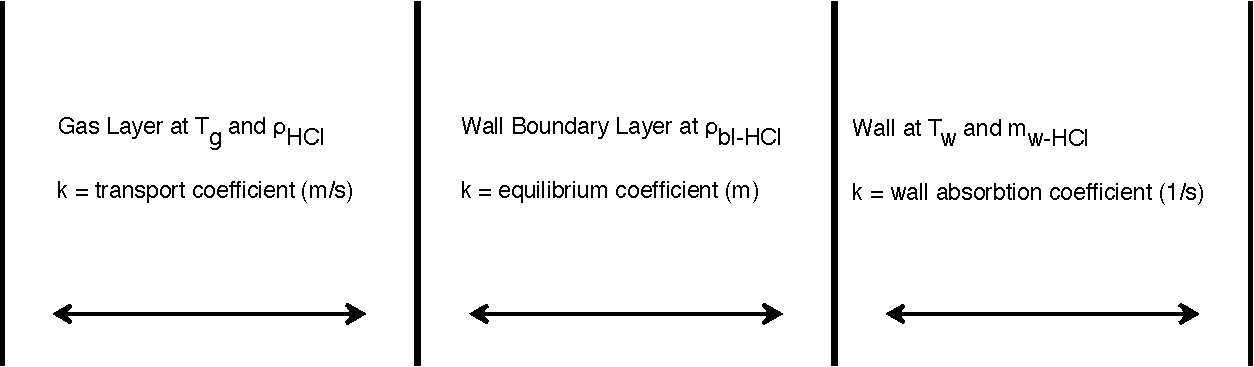
\includegraphics[width=5.0in]{FIGURES/Theory/HCl_Deposition}\\
\end{center}
\caption{Schematic of hydrogen chloride deposition region.}
 \label{fig:HCl_Deposition}
\end{figure}

The rate of addition of mass of hydrogen chloride to the gas layer is given by

\be \frac{d}{dt} m_{HCl} = source - k_c \brackets{\rho_{HCl} - \rho_{bl-HCl}} A_w \ee
where source is the production rate from the burning object plus flow from other compartments. For the wall concentration, the rate of addition is

\be \frac{d}{dt} d_{w-HCl} = k_c \brackets{\rho_{HCl} - \rho_{bl-HCl}} - k_s m_{w-HCl} \ee
where the concentration in the boundary layer, $\rho_{bl-HCl}$  is related to the wall surface concentration by the equilibrium constant $k_e$, by the relation $\rho_{bl-HCl} = d_{w-HCl} / k_e$. We never actually solve for the concentration in the boundary layer, but it is available, as is a boundary layer temperature if it were of interest.  The transfer coefficients are

\be k_c = \frac{\dot{q}}{\Delta T \rho_g c_p} \ee
\be k_e = \frac{b_1 e^{1500/T_w}}{1 + b_2 e^{1500/T_w} \rho_{HCl}} \brackets{1 + \frac{b_5 \brackets{\rho_{H_2O}}^{b_6}}{\brackets{\rho_{H_2O,sat} - \rho_{H_2O,g}}^{b_7}} } \ee
\be k_s = b_3 e^{-\brackets{\frac{b_4}{R T_w}}} \ee

The only values currently available  for these quantities are shown in table \ref{tab:HCL_Deposition} \cite{Galloway:1990}.  The ``$b$'' coefficients are parameters which are found by fitting experimental data to the above equations. These coefficients reproduce the adsorption and absorption of HCl reasonably well.  Note though that error bars for these coefficients have not been reported in the literature.

\begin{table}[t]
\begin{center}
\caption{Transfer coefficients for HCl deposition}
\label{tab:HCL_Deposition}
\begin{tabular}{| c | c | c | c | c | c | c | c |}
\hline
\multirow{2}{*}{Surface} & $b_1$ & $b_2$ & $b_3$ & $b_4$ & $b_5$ & $b_6$ & $b_7$ \\
 & (m) & (m\superscript{3}/kg) & (s\superscript{-1}) & (J/g mol) & (m\superscript{3}/kg)\superscript{$b_7 - b_6$} & (note a) & (note b) \\
 \hline
 Painted Gypsum & 0.0063 & 191.8 & 0.0587 & 7476 & 193 & 1.021 & 0.431 \\ \hline
 PMMA & $9.6 x 10^{-5}$ & 0.0137 & 0.0205 & 7476 & 29 & 1.0 & 0.431 \\ \hline
 Ceiling Tile & $4.0 x 10^{-3}$ & 0.0548 & 0.123 & 7476 & 30\superscript{a} & 1.0 & 0.431 \\ \hline
 Cement Block & $1.8 x 10^{-2}$ & 5.48 & 0.497 & 7476 & 30\superscript{a} & 1.0 & 0.431 \\  \hline
 Calcium Silicate Board & $1.9 x 10^{-2}$ & 0.137 & 0.030 & 7476 & 30\superscript{a} & 1.0 & 0.431 \\  \hline
\end{tabular}
\end{center}
a - very approximate value, insufficient data for high confidence value

b - non-dimensional
\end{table}

The experimental basis for poly(methyl methacrylate) and gypsum cover a sufficiently wide range of conditions that they should be usable in a variety of practical situations.  The parameters for the other surfaces do not have much experimental backing, and so their use should be limited to comparison purposes.




\backmatter


\bibliography{../Bibliography/CFAST_refs}
\addcontentsline{toc}{chapter}{References}

\appendix

\pagestyle{empty}

\chapter[Appendix A:  Calculation of Layer Height and the Average Upper and Lower Layer Temperatures]{Appendix A:  \\
\vspace{16 pt}
Calculation of Layer Height and the Average Upper and Lower Layer Temperatures}
\label{Appendix_layerheight}

% Test comment
% Test comment 2
% Test comment 3

Fire protection engineers often need to estimate the location of the interface between the hot, smoke-laden upper layer and the cooler lower layer in a burning compartment. Zone fire models such as CFAST compute this quantity directly, along with the average temperature of the upper and lower layers.  In an experimental test or a computational fluid dynamics (CFD) model like FDS \cite{FDS_Tech_Guide_5}, there are not two distinct zones, but rather a continuous profile of temperature. Nevertheless, methods have been developed to estimate layer height and average temperatures from a continuous vertical profile of temperature. One such method~\cite{Janssens:1992} is as follows: Consider a continuous function $T(z)$ defining temperature $T$ as a function of height above the floor $z$, where $z=0$ is the floor and $z=H$ is the ceiling. Define $T_u$ as the upper layer temperature, $T_l$ as the
lower layer temperature, and $z_{int}$ as the interface height. Compute the quantities:

\be (H-z_{int})\; T_u + z_{int} \; T_l = \int_0^H \; T(z) \; dz = I_1 \ee
\be (H-z_{int})\; \frac{1}{T_u} + z_{int} \; \frac{1}{T_l} = \int_0^H \; \frac{1}{T(z)} \; dz = I_2 \ee

Solve for $z_{int}$:

\be z_{int} = \frac{ T_l(I_1 \, I_2 - H^2)}{I_1+I_2 \, T_l^2 - 2\, T_l \, H} \ee

Let $T_l$ be the temperature in the lowest mesh cell and, using Simpson's Rule, perform the numerical integration of $I_1$ and $I_2$. $T_u$ is defined as the average upper layer temperature via

\be (H-z_{int})\; T_u = \int_{z_{int}}^H \; T(z) \; dz \ee

For experimental test data or CFD model output, the integral function of temperature as a function of height can be estimated empirically from a number of discrete data points. Further discussion of similar procedures can be found in Ref.~\cite{He:1998}.

\clearpage


\end{document}
